% lecture1.tex -- GENERATED by build_L1.py from L1_numbers.json; do not edit by hand.
\documentclass[10pt,aspectratio=169,t]{beamer}
% =============================================================================
% nn_preamble.tex -- shared Beamer preamble of Neural Networks and Deep Learning (NN)
% Used by every lecture: lectures/Lk/lecturek.tex does
%   \documentclass[10pt,aspectratio=169,t]{beamer}
%   % =============================================================================
% nn_preamble.tex -- shared Beamer preamble of Neural Networks and Deep Learning (NN)
% Used by every lecture: lectures/Lk/lecturek.tex does
%   \documentclass[10pt,aspectratio=169,t]{beamer}
%   % =============================================================================
% nn_preamble.tex -- shared Beamer preamble of Neural Networks and Deep Learning (NN)
% Used by every lecture: lectures/Lk/lecturek.tex does
%   \documentclass[10pt,aspectratio=169,t]{beamer}
%   \input{../common/nn_preamble}
%   \nnlecture{k}{Lecture title}
% Logos live in lectures/common/logos/, charts in lectures/Lk/charts/.
% Do NOT add \hfuzz / \vfuzz / \hbadness here: overfull boxes must be fixed, not hidden.
% =============================================================================

\usetheme{default}
\setbeamersize{text margin left=7mm, text margin right=7mm}

% ---------------------------------------------------------------- packages
\usepackage[utf8]{inputenc}
\usepackage[T1]{fontenc}
\usepackage{lmodern}
\usepackage{amsmath, amssymb}
\usepackage{mathtools}
\usepackage{bm}
\usepackage{tikz}
\usetikzlibrary{arrows.meta, positioning, calc, shapes.misc}
\usepackage{booktabs}
\usepackage{array}
\usepackage{graphicx}
\usepackage{colortbl}
\usepackage{xcolor}
\usepackage{multicol}
\hypersetup{colorlinks=true, linkcolor=MainBlue, urlcolor=MainBlue, citecolor=MainBlue}
\graphicspath{{../common/logos/}}   % charts are included with their language folder: charts/en/, charts/ro/

% ---------------------------------------------------------------- colours
\definecolor{MainBlue}{RGB}{26, 58, 110}
\definecolor{IDAred}{RGB}{205, 0, 0}
\definecolor{DarkGray}{RGB}{51, 51, 51}
\definecolor{FooterGray}{RGB}{100, 100, 100}
\definecolor{BlockGray}{RGB}{236, 238, 242}
\definecolor{KeynoteGray}{RGB}{218, 218, 218}
\definecolor{Crimson}{RGB}{190, 40, 50}
\definecolor{Forest}{RGB}{30, 110, 50}
\definecolor{Bitter}{RGB}{214, 150, 20}
% chart palette (same hex values and order as lectures/common/nn_plot.py SERIES)
\definecolor{Ser1}{HTML}{2A78D6}
\definecolor{Ser2}{HTML}{EB6834}
\definecolor{Ser3}{HTML}{1BAF7A}
\definecolor{Ser4}{HTML}{EDA100}
\definecolor{Ser5}{HTML}{E87BA4}
\definecolor{Ser6}{HTML}{008300}
\definecolor{Ser7}{HTML}{6250D6}
\definecolor{Ser8}{HTML}{E34948}

\setbeamertemplate{background}{%
  \begin{tikzpicture}[remember picture, overlay]
    \shade[shading=axis, shading angle=315, top color=white, bottom color=KeynoteGray]
      (current page.south west) rectangle (current page.north east);
  \end{tikzpicture}}
\setbeamercolor{background canvas}{bg=}
\setbeamercolor{structure}{fg=MainBlue}
\setbeamercolor{normal text}{fg=DarkGray}
\setbeamercolor{title}{fg=IDAred}
\setbeamercolor{frametitle}{fg=IDAred, bg=}
\setbeamercolor{block title}{bg=MainBlue, fg=white}
\setbeamercolor{block body}{bg=BlockGray, fg=DarkGray}
\setbeamercolor{block title alerted}{bg=Crimson, fg=white}
\setbeamercolor{block body alerted}{bg=Crimson!7, fg=DarkGray}
\setbeamercolor{block title example}{bg=Forest, fg=white}
\setbeamercolor{block body example}{bg=Forest!7, fg=DarkGray}
\setbeamercolor{item}{fg=MainBlue}
\setbeamerfont{frametitle}{size=\large, series=\bfseries}
\setbeamerfont{block title}{size=\small, series=\bfseries}
\setbeamertemplate{blocks}[rounded][shadow=false]
\setbeamertemplate{itemize item}{\color{MainBlue}$\boxdot$}
\setbeamertemplate{itemize subitem}{\color{MainBlue}\scriptsize$\blacktriangleright$}
% compact two-level lists: level 1 = main point, level 2 = details (no text outside bullets)
\setbeamerfont{itemize/enumerate subbody}{size=\footnotesize}
\setlength{\leftmargini}{1.1em}
\setlength{\leftmarginii}{1.1em}
\setbeamertemplate{itemize/enumerate body begin}{\setlength{\topsep}{0pt}\setlength{\partopsep}{0pt}\setlength{\parskip}{0pt}}
\setbeamertemplate{itemize/enumerate subbody begin}{\setlength{\topsep}{0pt}\setlength{\partopsep}{0pt}\setlength{\itemsep}{0pt}\vspace{-0.4ex}}

\setbeamertemplate{enumerate item}{\color{MainBlue}\insertenumlabel.}
\setlength{\leftmargini}{1.3em}
\setlength{\leftmarginii}{1.2em}
\setbeamertemplate{navigation symbols}{}
\setbeamertemplate{section in toc}{\color{MainBlue}$\blacktriangleright$~\inserttocsection}
\setbeamertemplate{caption}{\raggedright\insertcaption\par}
% frame subtitle = precise citation line under the claim title (Weron style)
\setbeamerfont{framesubtitle}{size=\footnotesize}
\setbeamercolor{framesubtitle}{fg=FooterGray}
% outline that reappears at every section with the current section highlighted
\setbeamertemplate{section in toc shaded}[default][35]
\setbeamertemplate{subsection in toc shaded}[default][35]
\setbeamertemplate{subsection in toc}{\leavevmode\leftskip=2.2em\color{DarkGray}\small\inserttocsubsection\par}
\AtBeginSection[]{{\begin{frame}{\txtoutline}\vspace{2mm}\small
  \tableofcontents[currentsection,hideothersubsections]\end{frame}}}

% ---------------------------------------------------------------- head and foot
\setbeamertemplate{headline}{%
  \vskip10pt%
  \hbox to \paperwidth{\hskip0.5cm%
    {\small\color{FooterGray}\renewcommand{\hyperlink}[2]{##2}\insertsectionhead}%
    \hfill\textcolor{FooterGray}{\small\insertframenumber}\hskip0.5cm}%
  \vskip4pt{\color{FooterGray}\hrule height 0.4pt}}
% footer as in the other courses (MFM, SFM): course name on the left, small sparkline on the right
\setbeamertemplate{footline}{%
  {\color{FooterGray}\hrule height 0.4pt}\vskip4pt%
  \hbox to \paperwidth{\hskip0.5cm%
    \textcolor{FooterGray}{\small\txtcourse}%
    \hfill\raisebox{-0.1em}{\begin{tikzpicture}[x=0.08em, y=0.08em, line width=0.4pt]
      \draw[FooterGray] (0,3) -- (1,4) -- (2,3.5) -- (3,5) -- (4,4) -- (5,6) -- (6,5.5) -- (7,4) -- (8,5) -- (9,7) -- (10,6) -- (11,5) -- (12,6.5) -- (13,8) -- (14,7) -- (15,6) -- (16,7.5) -- (17,9) -- (18,8) -- (19,7) -- (20,8.5) -- (21,10) -- (22,9) -- (23,8) -- (24,9.5);
    \end{tikzpicture}}\hskip0.5cm}%
  \vskip6pt}

% ---------------------------------------------------------------- title page
\defbeamertemplate*{title page}{nn}[1][]{%
  \vspace{0.15cm}
  \begin{center}
    \href{https://www.ase.ro}{
\includegraphics[height=0.9cm]{ase_logo.png}}\hspace{0.3cm}%
    \href{https://ipe.ro/new}{
\includegraphics[height=0.9cm]{acad_logo.png}}\hspace{0.3cm}%
    \href{https://theida.net}{
\includegraphics[height=0.9cm]{ida_logo.png}}\hspace{0.3cm}%
    \href{https://blockchain-research-center.com}{
\includegraphics[height=0.9cm]{brc_logo.png}}\hspace{0.3cm}%
    \href{https://www.ai4efin.ase.ro}{
\includegraphics[height=0.9cm]{ai4efin_logo.png}}\hspace{0.3cm}%
    \href{https://www.digital-finance-msca.com}{
\includegraphics[height=0.9cm]{msca_logo.png}}%
  \end{center}
  \vspace{0.45cm}
  \begin{center}
    \begin{minipage}{0.1\textwidth}\centering
      \href{https://quantlet.com}{
\includegraphics[height=0.9cm]{ql_logo.png}}\end{minipage}%
    \begin{minipage}{0.78\textwidth}\centering
      {\Large\bfseries\usebeamercolor[fg]{title}\inserttitle}\par\vspace{0.25cm}
      {\large\usebeamercolor[fg]{title}\insertsubtitle}\end{minipage}%
    \begin{minipage}{0.1\textwidth}\centering
      \href{https://quantinar.com}{
\includegraphics[height=0.9cm]{qr_logo.png}}\end{minipage}
  \end{center}
  \vfill
  \hspace{0.4cm}{\bfseries\insertauthor}\par\vspace{0.12cm}
  \hspace{0.4cm}\begin{minipage}[t]{0.92\textwidth}\raggedright\footnotesize\insertinstitute\end{minipage}
  \par\vspace{0.4cm}}

% ---------------------------------------------------------------- lecture metadata
\newcommand{\nnshort}{}
\newcommand{\nnnb}{notebooks}
\newcommand{\nnrepo}{https://github.com/danpele/NEURAL_BIZ/tree/main}
% language-dependent labels (English default; \nnromanian switches to Romanian, call it before \nnlecture)
\newcommand{\txtcourse}{Neural Networks and Deep Learning}
\newcommand{\txtlecture}{Lecture}
\newcommand{\txtoutline}{Outline}
\newcommand{\txtintuition}{In one sentence:}
\newcommand{\txtjob}{In practice:}
\newcommand{\txttry}{Experiment yourself:}
\newcommand{\txtwhere}{where}
\newcommand{\txtsim}{SIMULATED DATA (teaching illustration)}
\newcommand{\txtnbsuffix}{}
\newcommand{\txtinstitute}{Bucharest University of Economic Studies (ASE), Department of Statistics and Econometrics\\
    Romanian Academy, Institute for Economic Forecasting (IPE)\\
    IDA Institute Digital Assets \textbullet\ AI4EFin \textbullet\ MSCA Digital Finance}
\newcommand{\nnromanian}{%
  \renewcommand{\txtcourse}{Rețele neuronale și deep learning}%
  \renewcommand{\txtlecture}{Cursul}%
  \renewcommand{\txtoutline}{Cuprins}%
  \renewcommand{\txtintuition}{Pe scurt:}%
  \renewcommand{\txtjob}{În practică:}%
  \renewcommand{\txttry}{Exercițiu practic:}%
  \renewcommand{\txtwhere}{unde}%
  \renewcommand{\txtsim}{DATE SIMULATE (doar pentru ilustrare)}%
  \renewcommand{\txtnbsuffix}{\string_ro}%
  \renewcommand{\txtinstitute}{Academia de Studii Economice din București (ASE), Departamentul de Statistică și Econometrie\\
    Academia Română, Institutul de Prognoză Economică (IPE)\\
    IDA Institute Digital Assets \textbullet\ AI4EFin \textbullet\ MSCA Digital Finance}}
\newcommand{\nnlecture}[2]{%
  \renewcommand{\nnshort}{\txtlecture\ #1}%
  \renewcommand{\nnnb}{notebooks/L#1\string_notebook\txtnbsuffix.ipynb}%
  \title[NN]{\txtcourse}%
  \subtitle{\txtlecture\ #1: #2}%
  \author{Prof.\ dr.\ Daniel Traian PELE}%
  \institute{\txtinstitute}%
  \date{}}

% ---------------------------------------------------------------- teaching blocks (one message per frame)
% \intuition{one plain sentence}  ->  formula with every symbol defined  ->  real-data example  ->  \manager{one line}
\newcommand{\intuition}[1]{\begin{itemize}\item {\color{MainBlue}\textbf{\txtintuition}}~#1\end{itemize}\vspace{0.6mm}}
\newcommand{\manager}[1]{\colorbox{Forest!10}{\parbox{\dimexpr\linewidth-2\fboxsep\relax}{\footnotesize
  \begin{itemize}\setlength{\itemsep}{0pt}\item \textbf{\color{Forest}\txtjob}~#1\end{itemize}}}}
% Experiment yourself: pointer to the matching notebook section
\newcommand{\tryit}[1]{{\scriptsize\href{\nnrepo/\nnnb}{%
  \raisebox{-0.15em}{
\includegraphics[height=0.85em]{ql_logo.png}}\,\textbf{\txttry}~\color{MainBlue}#1}}}
% bottom row: manager line (left) + experiment pointer (right), pinned to the bottom of the frame
\newcommand{\bottomrow}[2]{\par\vfill\noindent\begin{minipage}[b]{0.72\linewidth}#1\end{minipage}\hfill
  \begin{minipage}[b]{0.26\linewidth}\raggedleft #2\end{minipage}\par\vspace{0.5mm}}
\newcommand{\where}[1]{{\footnotesize\textbf{\txtwhere}~#1\par}}

% ---------------------------------------------------------------- helpers
% chart source line under a figure: \chartsource{Source ...; period ...}
\newcommand{\chartsource}[1]{\par\vspace{1pt}{\scriptsize\color{FooterGray}#1\par}}
% link to code: \quantlet{label}{path inside the repo}
\newcommand{\quantlet}[2]{\par\vspace{1pt}\hfill\href{\nnrepo/#2}{%
  \raisebox{-0.15em}{
\includegraphics[height=0.75em]{ql_logo.png}}\textcolor{MainBlue}{\scriptsize\ #1}}}
% inline Quantlet link for the bottom-right corner of a frame: \qlink{label}{path inside the repo}
\newcommand{\qlink}[2]{{\scriptsize\href{\nnrepo/#2}{\raisebox{-0.15em}{
\includegraphics[height=0.85em]{ql_logo.png}}\,\textcolor{MainBlue}{#1}}}}
\newcommand{\simlabel}{\colorbox{Crimson!12}{\scriptsize\bfseries\color{Crimson}\txtsim}}
\newcommand{\E}{\mathbb{E}}
\newcommand{\Var}{\operatorname{Var}}
\newcommand{\Cov}{\operatorname{Cov}}
\newcommand{\Corr}{\operatorname{Corr}}
\newcommand{\asinh}{\operatorname{asinh}}
\newcommand{\iid}{\overset{\text{i.i.d.}}{\sim}}
\newcommand{\EUR}{EUR}
% deep-learning notation (Bishop & Bishop, 2024): vectors bold lower case, matrices bold upper case
\newcommand{\R}{\mathbb{R}}
\newcommand{\vx}{\mathbf{x}}
\newcommand{\vy}{\mathbf{y}}
\newcommand{\vz}{\mathbf{z}}
\newcommand{\vh}{\mathbf{h}}
\newcommand{\vw}{\mathbf{w}}
\newcommand{\vb}{\mathbf{b}}
\newcommand{\mW}{\mathbf{W}}
\newcommand{\mX}{\mathbf{X}}
\newcommand{\btheta}{\boldsymbol{\theta}}
\newcommand{\loss}{\mathcal{L}}
\newcommand{\dataset}{\mathcal{D}}
\DeclareMathOperator*{\argmin}{arg\,min}
\DeclareMathOperator*{\argmax}{arg\,max}
\DeclareMathOperator{\softmax}{softmax}
\DeclareMathOperator{\ReLU}{ReLU}
\DeclareMathOperator{\sigm}{\sigma}

%   \nnlecture{k}{Lecture title}
% Logos live in lectures/common/logos/, charts in lectures/Lk/charts/.
% Do NOT add \hfuzz / \vfuzz / \hbadness here: overfull boxes must be fixed, not hidden.
% =============================================================================

\usetheme{default}
\setbeamersize{text margin left=7mm, text margin right=7mm}

% ---------------------------------------------------------------- packages
\usepackage[utf8]{inputenc}
\usepackage[T1]{fontenc}
\usepackage{lmodern}
\usepackage{amsmath, amssymb}
\usepackage{mathtools}
\usepackage{bm}
\usepackage{tikz}
\usetikzlibrary{arrows.meta, positioning, calc, shapes.misc}
\usepackage{booktabs}
\usepackage{array}
\usepackage{graphicx}
\usepackage{colortbl}
\usepackage{xcolor}
\usepackage{multicol}
\hypersetup{colorlinks=true, linkcolor=MainBlue, urlcolor=MainBlue, citecolor=MainBlue}
\graphicspath{{../common/logos/}}   % charts are included with their language folder: charts/en/, charts/ro/

% ---------------------------------------------------------------- colours
\definecolor{MainBlue}{RGB}{26, 58, 110}
\definecolor{IDAred}{RGB}{205, 0, 0}
\definecolor{DarkGray}{RGB}{51, 51, 51}
\definecolor{FooterGray}{RGB}{100, 100, 100}
\definecolor{BlockGray}{RGB}{236, 238, 242}
\definecolor{KeynoteGray}{RGB}{218, 218, 218}
\definecolor{Crimson}{RGB}{190, 40, 50}
\definecolor{Forest}{RGB}{30, 110, 50}
\definecolor{Bitter}{RGB}{214, 150, 20}
% chart palette (same hex values and order as lectures/common/nn_plot.py SERIES)
\definecolor{Ser1}{HTML}{2A78D6}
\definecolor{Ser2}{HTML}{EB6834}
\definecolor{Ser3}{HTML}{1BAF7A}
\definecolor{Ser4}{HTML}{EDA100}
\definecolor{Ser5}{HTML}{E87BA4}
\definecolor{Ser6}{HTML}{008300}
\definecolor{Ser7}{HTML}{6250D6}
\definecolor{Ser8}{HTML}{E34948}

\setbeamertemplate{background}{%
  \begin{tikzpicture}[remember picture, overlay]
    \shade[shading=axis, shading angle=315, top color=white, bottom color=KeynoteGray]
      (current page.south west) rectangle (current page.north east);
  \end{tikzpicture}}
\setbeamercolor{background canvas}{bg=}
\setbeamercolor{structure}{fg=MainBlue}
\setbeamercolor{normal text}{fg=DarkGray}
\setbeamercolor{title}{fg=IDAred}
\setbeamercolor{frametitle}{fg=IDAred, bg=}
\setbeamercolor{block title}{bg=MainBlue, fg=white}
\setbeamercolor{block body}{bg=BlockGray, fg=DarkGray}
\setbeamercolor{block title alerted}{bg=Crimson, fg=white}
\setbeamercolor{block body alerted}{bg=Crimson!7, fg=DarkGray}
\setbeamercolor{block title example}{bg=Forest, fg=white}
\setbeamercolor{block body example}{bg=Forest!7, fg=DarkGray}
\setbeamercolor{item}{fg=MainBlue}
\setbeamerfont{frametitle}{size=\large, series=\bfseries}
\setbeamerfont{block title}{size=\small, series=\bfseries}
\setbeamertemplate{blocks}[rounded][shadow=false]
\setbeamertemplate{itemize item}{\color{MainBlue}$\boxdot$}
\setbeamertemplate{itemize subitem}{\color{MainBlue}\scriptsize$\blacktriangleright$}
% compact two-level lists: level 1 = main point, level 2 = details (no text outside bullets)
\setbeamerfont{itemize/enumerate subbody}{size=\footnotesize}
\setlength{\leftmargini}{1.1em}
\setlength{\leftmarginii}{1.1em}
\setbeamertemplate{itemize/enumerate body begin}{\setlength{\topsep}{0pt}\setlength{\partopsep}{0pt}\setlength{\parskip}{0pt}}
\setbeamertemplate{itemize/enumerate subbody begin}{\setlength{\topsep}{0pt}\setlength{\partopsep}{0pt}\setlength{\itemsep}{0pt}\vspace{-0.4ex}}

\setbeamertemplate{enumerate item}{\color{MainBlue}\insertenumlabel.}
\setlength{\leftmargini}{1.3em}
\setlength{\leftmarginii}{1.2em}
\setbeamertemplate{navigation symbols}{}
\setbeamertemplate{section in toc}{\color{MainBlue}$\blacktriangleright$~\inserttocsection}
\setbeamertemplate{caption}{\raggedright\insertcaption\par}
% frame subtitle = precise citation line under the claim title (Weron style)
\setbeamerfont{framesubtitle}{size=\footnotesize}
\setbeamercolor{framesubtitle}{fg=FooterGray}
% outline that reappears at every section with the current section highlighted
\setbeamertemplate{section in toc shaded}[default][35]
\setbeamertemplate{subsection in toc shaded}[default][35]
\setbeamertemplate{subsection in toc}{\leavevmode\leftskip=2.2em\color{DarkGray}\small\inserttocsubsection\par}
\AtBeginSection[]{{\begin{frame}{\txtoutline}\vspace{2mm}\small
  \tableofcontents[currentsection,hideothersubsections]\end{frame}}}

% ---------------------------------------------------------------- head and foot
\setbeamertemplate{headline}{%
  \vskip10pt%
  \hbox to \paperwidth{\hskip0.5cm%
    {\small\color{FooterGray}\renewcommand{\hyperlink}[2]{##2}\insertsectionhead}%
    \hfill\textcolor{FooterGray}{\small\insertframenumber}\hskip0.5cm}%
  \vskip4pt{\color{FooterGray}\hrule height 0.4pt}}
% footer as in the other courses (MFM, SFM): course name on the left, small sparkline on the right
\setbeamertemplate{footline}{%
  {\color{FooterGray}\hrule height 0.4pt}\vskip4pt%
  \hbox to \paperwidth{\hskip0.5cm%
    \textcolor{FooterGray}{\small\txtcourse}%
    \hfill\raisebox{-0.1em}{\begin{tikzpicture}[x=0.08em, y=0.08em, line width=0.4pt]
      \draw[FooterGray] (0,3) -- (1,4) -- (2,3.5) -- (3,5) -- (4,4) -- (5,6) -- (6,5.5) -- (7,4) -- (8,5) -- (9,7) -- (10,6) -- (11,5) -- (12,6.5) -- (13,8) -- (14,7) -- (15,6) -- (16,7.5) -- (17,9) -- (18,8) -- (19,7) -- (20,8.5) -- (21,10) -- (22,9) -- (23,8) -- (24,9.5);
    \end{tikzpicture}}\hskip0.5cm}%
  \vskip6pt}

% ---------------------------------------------------------------- title page
\defbeamertemplate*{title page}{nn}[1][]{%
  \vspace{0.15cm}
  \begin{center}
    \href{https://www.ase.ro}{
\includegraphics[height=0.9cm]{ase_logo.png}}\hspace{0.3cm}%
    \href{https://ipe.ro/new}{
\includegraphics[height=0.9cm]{acad_logo.png}}\hspace{0.3cm}%
    \href{https://theida.net}{
\includegraphics[height=0.9cm]{ida_logo.png}}\hspace{0.3cm}%
    \href{https://blockchain-research-center.com}{
\includegraphics[height=0.9cm]{brc_logo.png}}\hspace{0.3cm}%
    \href{https://www.ai4efin.ase.ro}{
\includegraphics[height=0.9cm]{ai4efin_logo.png}}\hspace{0.3cm}%
    \href{https://www.digital-finance-msca.com}{
\includegraphics[height=0.9cm]{msca_logo.png}}%
  \end{center}
  \vspace{0.45cm}
  \begin{center}
    \begin{minipage}{0.1\textwidth}\centering
      \href{https://quantlet.com}{
\includegraphics[height=0.9cm]{ql_logo.png}}\end{minipage}%
    \begin{minipage}{0.78\textwidth}\centering
      {\Large\bfseries\usebeamercolor[fg]{title}\inserttitle}\par\vspace{0.25cm}
      {\large\usebeamercolor[fg]{title}\insertsubtitle}\end{minipage}%
    \begin{minipage}{0.1\textwidth}\centering
      \href{https://quantinar.com}{
\includegraphics[height=0.9cm]{qr_logo.png}}\end{minipage}
  \end{center}
  \vfill
  \hspace{0.4cm}{\bfseries\insertauthor}\par\vspace{0.12cm}
  \hspace{0.4cm}\begin{minipage}[t]{0.92\textwidth}\raggedright\footnotesize\insertinstitute\end{minipage}
  \par\vspace{0.4cm}}

% ---------------------------------------------------------------- lecture metadata
\newcommand{\nnshort}{}
\newcommand{\nnnb}{notebooks}
\newcommand{\nnrepo}{https://github.com/danpele/NEURAL_BIZ/tree/main}
% language-dependent labels (English default; \nnromanian switches to Romanian, call it before \nnlecture)
\newcommand{\txtcourse}{Neural Networks and Deep Learning}
\newcommand{\txtlecture}{Lecture}
\newcommand{\txtoutline}{Outline}
\newcommand{\txtintuition}{In one sentence:}
\newcommand{\txtjob}{In practice:}
\newcommand{\txttry}{Experiment yourself:}
\newcommand{\txtwhere}{where}
\newcommand{\txtsim}{SIMULATED DATA (teaching illustration)}
\newcommand{\txtnbsuffix}{}
\newcommand{\txtinstitute}{Bucharest University of Economic Studies (ASE), Department of Statistics and Econometrics\\
    Romanian Academy, Institute for Economic Forecasting (IPE)\\
    IDA Institute Digital Assets \textbullet\ AI4EFin \textbullet\ MSCA Digital Finance}
\newcommand{\nnromanian}{%
  \renewcommand{\txtcourse}{Rețele neuronale și deep learning}%
  \renewcommand{\txtlecture}{Cursul}%
  \renewcommand{\txtoutline}{Cuprins}%
  \renewcommand{\txtintuition}{Pe scurt:}%
  \renewcommand{\txtjob}{În practică:}%
  \renewcommand{\txttry}{Exercițiu practic:}%
  \renewcommand{\txtwhere}{unde}%
  \renewcommand{\txtsim}{DATE SIMULATE (doar pentru ilustrare)}%
  \renewcommand{\txtnbsuffix}{\string_ro}%
  \renewcommand{\txtinstitute}{Academia de Studii Economice din București (ASE), Departamentul de Statistică și Econometrie\\
    Academia Română, Institutul de Prognoză Economică (IPE)\\
    IDA Institute Digital Assets \textbullet\ AI4EFin \textbullet\ MSCA Digital Finance}}
\newcommand{\nnlecture}[2]{%
  \renewcommand{\nnshort}{\txtlecture\ #1}%
  \renewcommand{\nnnb}{notebooks/L#1\string_notebook\txtnbsuffix.ipynb}%
  \title[NN]{\txtcourse}%
  \subtitle{\txtlecture\ #1: #2}%
  \author{Prof.\ dr.\ Daniel Traian PELE}%
  \institute{\txtinstitute}%
  \date{}}

% ---------------------------------------------------------------- teaching blocks (one message per frame)
% \intuition{one plain sentence}  ->  formula with every symbol defined  ->  real-data example  ->  \manager{one line}
\newcommand{\intuition}[1]{\begin{itemize}\item {\color{MainBlue}\textbf{\txtintuition}}~#1\end{itemize}\vspace{0.6mm}}
\newcommand{\manager}[1]{\colorbox{Forest!10}{\parbox{\dimexpr\linewidth-2\fboxsep\relax}{\footnotesize
  \begin{itemize}\setlength{\itemsep}{0pt}\item \textbf{\color{Forest}\txtjob}~#1\end{itemize}}}}
% Experiment yourself: pointer to the matching notebook section
\newcommand{\tryit}[1]{{\scriptsize\href{\nnrepo/\nnnb}{%
  \raisebox{-0.15em}{
\includegraphics[height=0.85em]{ql_logo.png}}\,\textbf{\txttry}~\color{MainBlue}#1}}}
% bottom row: manager line (left) + experiment pointer (right), pinned to the bottom of the frame
\newcommand{\bottomrow}[2]{\par\vfill\noindent\begin{minipage}[b]{0.72\linewidth}#1\end{minipage}\hfill
  \begin{minipage}[b]{0.26\linewidth}\raggedleft #2\end{minipage}\par\vspace{0.5mm}}
\newcommand{\where}[1]{{\footnotesize\textbf{\txtwhere}~#1\par}}

% ---------------------------------------------------------------- helpers
% chart source line under a figure: \chartsource{Source ...; period ...}
\newcommand{\chartsource}[1]{\par\vspace{1pt}{\scriptsize\color{FooterGray}#1\par}}
% link to code: \quantlet{label}{path inside the repo}
\newcommand{\quantlet}[2]{\par\vspace{1pt}\hfill\href{\nnrepo/#2}{%
  \raisebox{-0.15em}{
\includegraphics[height=0.75em]{ql_logo.png}}\textcolor{MainBlue}{\scriptsize\ #1}}}
% inline Quantlet link for the bottom-right corner of a frame: \qlink{label}{path inside the repo}
\newcommand{\qlink}[2]{{\scriptsize\href{\nnrepo/#2}{\raisebox{-0.15em}{
\includegraphics[height=0.85em]{ql_logo.png}}\,\textcolor{MainBlue}{#1}}}}
\newcommand{\simlabel}{\colorbox{Crimson!12}{\scriptsize\bfseries\color{Crimson}\txtsim}}
\newcommand{\E}{\mathbb{E}}
\newcommand{\Var}{\operatorname{Var}}
\newcommand{\Cov}{\operatorname{Cov}}
\newcommand{\Corr}{\operatorname{Corr}}
\newcommand{\asinh}{\operatorname{asinh}}
\newcommand{\iid}{\overset{\text{i.i.d.}}{\sim}}
\newcommand{\EUR}{EUR}
% deep-learning notation (Bishop & Bishop, 2024): vectors bold lower case, matrices bold upper case
\newcommand{\R}{\mathbb{R}}
\newcommand{\vx}{\mathbf{x}}
\newcommand{\vy}{\mathbf{y}}
\newcommand{\vz}{\mathbf{z}}
\newcommand{\vh}{\mathbf{h}}
\newcommand{\vw}{\mathbf{w}}
\newcommand{\vb}{\mathbf{b}}
\newcommand{\mW}{\mathbf{W}}
\newcommand{\mX}{\mathbf{X}}
\newcommand{\btheta}{\boldsymbol{\theta}}
\newcommand{\loss}{\mathcal{L}}
\newcommand{\dataset}{\mathcal{D}}
\DeclareMathOperator*{\argmin}{arg\,min}
\DeclareMathOperator*{\argmax}{arg\,max}
\DeclareMathOperator{\softmax}{softmax}
\DeclareMathOperator{\ReLU}{ReLU}
\DeclareMathOperator{\sigm}{\sigma}

%   \nnlecture{k}{Lecture title}
% Logos live in lectures/common/logos/, charts in lectures/Lk/charts/.
% Do NOT add \hfuzz / \vfuzz / \hbadness here: overfull boxes must be fixed, not hidden.
% =============================================================================

\usetheme{default}
\setbeamersize{text margin left=7mm, text margin right=7mm}

% ---------------------------------------------------------------- packages
\usepackage[utf8]{inputenc}
\usepackage[T1]{fontenc}
\usepackage{lmodern}
\usepackage{amsmath, amssymb}
\usepackage{mathtools}
\usepackage{bm}
\usepackage{tikz}
\usetikzlibrary{arrows.meta, positioning, calc, shapes.misc}
\usepackage{booktabs}
\usepackage{array}
\usepackage{graphicx}
\usepackage{colortbl}
\usepackage{xcolor}
\usepackage{multicol}
\hypersetup{colorlinks=true, linkcolor=MainBlue, urlcolor=MainBlue, citecolor=MainBlue}
\graphicspath{{../common/logos/}}   % charts are included with their language folder: charts/en/, charts/ro/

% ---------------------------------------------------------------- colours
\definecolor{MainBlue}{RGB}{26, 58, 110}
\definecolor{IDAred}{RGB}{205, 0, 0}
\definecolor{DarkGray}{RGB}{51, 51, 51}
\definecolor{FooterGray}{RGB}{100, 100, 100}
\definecolor{BlockGray}{RGB}{236, 238, 242}
\definecolor{KeynoteGray}{RGB}{218, 218, 218}
\definecolor{Crimson}{RGB}{190, 40, 50}
\definecolor{Forest}{RGB}{30, 110, 50}
\definecolor{Bitter}{RGB}{214, 150, 20}
% chart palette (same hex values and order as lectures/common/nn_plot.py SERIES)
\definecolor{Ser1}{HTML}{2A78D6}
\definecolor{Ser2}{HTML}{EB6834}
\definecolor{Ser3}{HTML}{1BAF7A}
\definecolor{Ser4}{HTML}{EDA100}
\definecolor{Ser5}{HTML}{E87BA4}
\definecolor{Ser6}{HTML}{008300}
\definecolor{Ser7}{HTML}{6250D6}
\definecolor{Ser8}{HTML}{E34948}

\setbeamertemplate{background}{%
  \begin{tikzpicture}[remember picture, overlay]
    \shade[shading=axis, shading angle=315, top color=white, bottom color=KeynoteGray]
      (current page.south west) rectangle (current page.north east);
  \end{tikzpicture}}
\setbeamercolor{background canvas}{bg=}
\setbeamercolor{structure}{fg=MainBlue}
\setbeamercolor{normal text}{fg=DarkGray}
\setbeamercolor{title}{fg=IDAred}
\setbeamercolor{frametitle}{fg=IDAred, bg=}
\setbeamercolor{block title}{bg=MainBlue, fg=white}
\setbeamercolor{block body}{bg=BlockGray, fg=DarkGray}
\setbeamercolor{block title alerted}{bg=Crimson, fg=white}
\setbeamercolor{block body alerted}{bg=Crimson!7, fg=DarkGray}
\setbeamercolor{block title example}{bg=Forest, fg=white}
\setbeamercolor{block body example}{bg=Forest!7, fg=DarkGray}
\setbeamercolor{item}{fg=MainBlue}
\setbeamerfont{frametitle}{size=\large, series=\bfseries}
\setbeamerfont{block title}{size=\small, series=\bfseries}
\setbeamertemplate{blocks}[rounded][shadow=false]
\setbeamertemplate{itemize item}{\color{MainBlue}$\boxdot$}
\setbeamertemplate{itemize subitem}{\color{MainBlue}\scriptsize$\blacktriangleright$}
% compact two-level lists: level 1 = main point, level 2 = details (no text outside bullets)
\setbeamerfont{itemize/enumerate subbody}{size=\footnotesize}
\setlength{\leftmargini}{1.1em}
\setlength{\leftmarginii}{1.1em}
\setbeamertemplate{itemize/enumerate body begin}{\setlength{\topsep}{0pt}\setlength{\partopsep}{0pt}\setlength{\parskip}{0pt}}
\setbeamertemplate{itemize/enumerate subbody begin}{\setlength{\topsep}{0pt}\setlength{\partopsep}{0pt}\setlength{\itemsep}{0pt}\vspace{-0.4ex}}

\setbeamertemplate{enumerate item}{\color{MainBlue}\insertenumlabel.}
\setlength{\leftmargini}{1.3em}
\setlength{\leftmarginii}{1.2em}
\setbeamertemplate{navigation symbols}{}
\setbeamertemplate{section in toc}{\color{MainBlue}$\blacktriangleright$~\inserttocsection}
\setbeamertemplate{caption}{\raggedright\insertcaption\par}
% frame subtitle = precise citation line under the claim title (Weron style)
\setbeamerfont{framesubtitle}{size=\footnotesize}
\setbeamercolor{framesubtitle}{fg=FooterGray}
% outline that reappears at every section with the current section highlighted
\setbeamertemplate{section in toc shaded}[default][35]
\setbeamertemplate{subsection in toc shaded}[default][35]
\setbeamertemplate{subsection in toc}{\leavevmode\leftskip=2.2em\color{DarkGray}\small\inserttocsubsection\par}
\AtBeginSection[]{{\begin{frame}{\txtoutline}\vspace{2mm}\small
  \tableofcontents[currentsection,hideothersubsections]\end{frame}}}

% ---------------------------------------------------------------- head and foot
\setbeamertemplate{headline}{%
  \vskip10pt%
  \hbox to \paperwidth{\hskip0.5cm%
    {\small\color{FooterGray}\renewcommand{\hyperlink}[2]{##2}\insertsectionhead}%
    \hfill\textcolor{FooterGray}{\small\insertframenumber}\hskip0.5cm}%
  \vskip4pt{\color{FooterGray}\hrule height 0.4pt}}
% footer as in the other courses (MFM, SFM): course name on the left, small sparkline on the right
\setbeamertemplate{footline}{%
  {\color{FooterGray}\hrule height 0.4pt}\vskip4pt%
  \hbox to \paperwidth{\hskip0.5cm%
    \textcolor{FooterGray}{\small\txtcourse}%
    \hfill\raisebox{-0.1em}{\begin{tikzpicture}[x=0.08em, y=0.08em, line width=0.4pt]
      \draw[FooterGray] (0,3) -- (1,4) -- (2,3.5) -- (3,5) -- (4,4) -- (5,6) -- (6,5.5) -- (7,4) -- (8,5) -- (9,7) -- (10,6) -- (11,5) -- (12,6.5) -- (13,8) -- (14,7) -- (15,6) -- (16,7.5) -- (17,9) -- (18,8) -- (19,7) -- (20,8.5) -- (21,10) -- (22,9) -- (23,8) -- (24,9.5);
    \end{tikzpicture}}\hskip0.5cm}%
  \vskip6pt}

% ---------------------------------------------------------------- title page
\defbeamertemplate*{title page}{nn}[1][]{%
  \vspace{0.15cm}
  \begin{center}
    \href{https://www.ase.ro}{
\includegraphics[height=0.9cm]{ase_logo.png}}\hspace{0.3cm}%
    \href{https://ipe.ro/new}{
\includegraphics[height=0.9cm]{acad_logo.png}}\hspace{0.3cm}%
    \href{https://theida.net}{
\includegraphics[height=0.9cm]{ida_logo.png}}\hspace{0.3cm}%
    \href{https://blockchain-research-center.com}{
\includegraphics[height=0.9cm]{brc_logo.png}}\hspace{0.3cm}%
    \href{https://www.ai4efin.ase.ro}{
\includegraphics[height=0.9cm]{ai4efin_logo.png}}\hspace{0.3cm}%
    \href{https://www.digital-finance-msca.com}{
\includegraphics[height=0.9cm]{msca_logo.png}}%
  \end{center}
  \vspace{0.45cm}
  \begin{center}
    \begin{minipage}{0.1\textwidth}\centering
      \href{https://quantlet.com}{
\includegraphics[height=0.9cm]{ql_logo.png}}\end{minipage}%
    \begin{minipage}{0.78\textwidth}\centering
      {\Large\bfseries\usebeamercolor[fg]{title}\inserttitle}\par\vspace{0.25cm}
      {\large\usebeamercolor[fg]{title}\insertsubtitle}\end{minipage}%
    \begin{minipage}{0.1\textwidth}\centering
      \href{https://quantinar.com}{
\includegraphics[height=0.9cm]{qr_logo.png}}\end{minipage}
  \end{center}
  \vfill
  \hspace{0.4cm}{\bfseries\insertauthor}\par\vspace{0.12cm}
  \hspace{0.4cm}\begin{minipage}[t]{0.92\textwidth}\raggedright\footnotesize\insertinstitute\end{minipage}
  \par\vspace{0.4cm}}

% ---------------------------------------------------------------- lecture metadata
\newcommand{\nnshort}{}
\newcommand{\nnnb}{notebooks}
\newcommand{\nnrepo}{https://github.com/danpele/NEURAL_BIZ/tree/main}
% language-dependent labels (English default; \nnromanian switches to Romanian, call it before \nnlecture)
\newcommand{\txtcourse}{Neural Networks and Deep Learning}
\newcommand{\txtlecture}{Lecture}
\newcommand{\txtoutline}{Outline}
\newcommand{\txtintuition}{In one sentence:}
\newcommand{\txtjob}{In practice:}
\newcommand{\txttry}{Experiment yourself:}
\newcommand{\txtwhere}{where}
\newcommand{\txtsim}{SIMULATED DATA (teaching illustration)}
\newcommand{\txtnbsuffix}{}
\newcommand{\txtinstitute}{Bucharest University of Economic Studies (ASE), Department of Statistics and Econometrics\\
    Romanian Academy, Institute for Economic Forecasting (IPE)\\
    IDA Institute Digital Assets \textbullet\ AI4EFin \textbullet\ MSCA Digital Finance}
\newcommand{\nnromanian}{%
  \renewcommand{\txtcourse}{Rețele neuronale și deep learning}%
  \renewcommand{\txtlecture}{Cursul}%
  \renewcommand{\txtoutline}{Cuprins}%
  \renewcommand{\txtintuition}{Pe scurt:}%
  \renewcommand{\txtjob}{În practică:}%
  \renewcommand{\txttry}{Exercițiu practic:}%
  \renewcommand{\txtwhere}{unde}%
  \renewcommand{\txtsim}{DATE SIMULATE (doar pentru ilustrare)}%
  \renewcommand{\txtnbsuffix}{\string_ro}%
  \renewcommand{\txtinstitute}{Academia de Studii Economice din București (ASE), Departamentul de Statistică și Econometrie\\
    Academia Română, Institutul de Prognoză Economică (IPE)\\
    IDA Institute Digital Assets \textbullet\ AI4EFin \textbullet\ MSCA Digital Finance}}
\newcommand{\nnlecture}[2]{%
  \renewcommand{\nnshort}{\txtlecture\ #1}%
  \renewcommand{\nnnb}{notebooks/L#1\string_notebook\txtnbsuffix.ipynb}%
  \title[NN]{\txtcourse}%
  \subtitle{\txtlecture\ #1: #2}%
  \author{Prof.\ dr.\ Daniel Traian PELE}%
  \institute{\txtinstitute}%
  \date{}}

% ---------------------------------------------------------------- teaching blocks (one message per frame)
% \intuition{one plain sentence}  ->  formula with every symbol defined  ->  real-data example  ->  \manager{one line}
\newcommand{\intuition}[1]{\begin{itemize}\item {\color{MainBlue}\textbf{\txtintuition}}~#1\end{itemize}\vspace{0.6mm}}
\newcommand{\manager}[1]{\colorbox{Forest!10}{\parbox{\dimexpr\linewidth-2\fboxsep\relax}{\footnotesize
  \begin{itemize}\setlength{\itemsep}{0pt}\item \textbf{\color{Forest}\txtjob}~#1\end{itemize}}}}
% Experiment yourself: pointer to the matching notebook section
\newcommand{\tryit}[1]{{\scriptsize\href{\nnrepo/\nnnb}{%
  \raisebox{-0.15em}{
\includegraphics[height=0.85em]{ql_logo.png}}\,\textbf{\txttry}~\color{MainBlue}#1}}}
% bottom row: manager line (left) + experiment pointer (right), pinned to the bottom of the frame
\newcommand{\bottomrow}[2]{\par\vfill\noindent\begin{minipage}[b]{0.72\linewidth}#1\end{minipage}\hfill
  \begin{minipage}[b]{0.26\linewidth}\raggedleft #2\end{minipage}\par\vspace{0.5mm}}
\newcommand{\where}[1]{{\footnotesize\textbf{\txtwhere}~#1\par}}

% ---------------------------------------------------------------- helpers
% chart source line under a figure: \chartsource{Source ...; period ...}
\newcommand{\chartsource}[1]{\par\vspace{1pt}{\scriptsize\color{FooterGray}#1\par}}
% link to code: \quantlet{label}{path inside the repo}
\newcommand{\quantlet}[2]{\par\vspace{1pt}\hfill\href{\nnrepo/#2}{%
  \raisebox{-0.15em}{
\includegraphics[height=0.75em]{ql_logo.png}}\textcolor{MainBlue}{\scriptsize\ #1}}}
% inline Quantlet link for the bottom-right corner of a frame: \qlink{label}{path inside the repo}
\newcommand{\qlink}[2]{{\scriptsize\href{\nnrepo/#2}{\raisebox{-0.15em}{
\includegraphics[height=0.85em]{ql_logo.png}}\,\textcolor{MainBlue}{#1}}}}
\newcommand{\simlabel}{\colorbox{Crimson!12}{\scriptsize\bfseries\color{Crimson}\txtsim}}
\newcommand{\E}{\mathbb{E}}
\newcommand{\Var}{\operatorname{Var}}
\newcommand{\Cov}{\operatorname{Cov}}
\newcommand{\Corr}{\operatorname{Corr}}
\newcommand{\asinh}{\operatorname{asinh}}
\newcommand{\iid}{\overset{\text{i.i.d.}}{\sim}}
\newcommand{\EUR}{EUR}
% deep-learning notation (Bishop & Bishop, 2024): vectors bold lower case, matrices bold upper case
\newcommand{\R}{\mathbb{R}}
\newcommand{\vx}{\mathbf{x}}
\newcommand{\vy}{\mathbf{y}}
\newcommand{\vz}{\mathbf{z}}
\newcommand{\vh}{\mathbf{h}}
\newcommand{\vw}{\mathbf{w}}
\newcommand{\vb}{\mathbf{b}}
\newcommand{\mW}{\mathbf{W}}
\newcommand{\mX}{\mathbf{X}}
\newcommand{\btheta}{\boldsymbol{\theta}}
\newcommand{\loss}{\mathcal{L}}
\newcommand{\dataset}{\mathcal{D}}
\DeclareMathOperator*{\argmin}{arg\,min}
\DeclareMathOperator*{\argmax}{arg\,max}
\DeclareMathOperator{\softmax}{softmax}
\DeclareMathOperator{\ReLU}{ReLU}
\DeclareMathOperator{\sigm}{\sigma}

\nnlecture{1}{Deep learning for business: from linear models to the perceptron and the multilayer perceptron (MLP)}
\begin{document}
{\setbeamertemplate{headline}{}\setbeamertemplate{footline}{}
\begin{frame}\titlepage\end{frame}}
% END-FRONT-MATTER

\begin{frame}{Learning objectives}
\small
\begin{itemize}\setlength{\itemsep}{4pt}
  \item Place deep learning among the tools of a business analyst: where it creates value and where a linear model is enough.
  \item Write linear and logistic regression as one-neuron networks, with their loss as a likelihood.
  \item Explain Rosenblatt's perceptron, its learning rule, its convergence theorem and its limit (the exclusive or (XOR) problem).
  \item Build a multilayer perceptron (MLP): forward pass, activation functions, number of parameters, universal approximation.
  \item Compare an MLP with logistic regression and gradient boosting for credit scoring on real data, with costs and uncertainty.
\end{itemize}
\end{frame}

% BEGIN-ABBR

\begin{frame}{Abbreviations}
\small
\vspace{-1mm}\begin{columns}[T,onlytextwidth]
\begin{column}{0.49\textwidth}{\scriptsize\renewcommand{\arraystretch}{0.96}\begin{tabular}{@{}>{\bfseries}l@{\ \ }p{0.74\linewidth}@{}}AI & artificial intelligence\\
AUC & area under the receiver operating characteristic curve\\
CPU & central processing unit\\
DM & Deutsche Mark\\
ES & expected shortfall\\
GELU & Gaussian error linear unit\\
GNN & graph neural network\\
GPU & graphics processing unit\\
GraphSAGE & graph sample and aggregate (a GNN architecture)\\
HMEQ & home equity loans dataset\\
ICBE & International Conference on Business Excellence\\
IEEE-CIS & Institute of Electrical and Electronics Engineers, Computational Intelligence Society\\
LLM & large language model\\
MLP & multilayer perceptron\\\end{tabular}}\end{column}
\begin{column}{0.49\textwidth}{\scriptsize\renewcommand{\arraystretch}{0.96}\begin{tabular}{@{}>{\bfseries}l@{\ \ }p{0.74\linewidth}@{}}MSE & mean squared error\\
PD & probability of default\\
ReLU & rectified linear unit\\
ROC & receiver operating characteristic\\
SGD & stochastic gradient descent\\
SHAP & Shapley additive explanations\\
UCI & University of California, Irvine (Machine Learning Repository)\\
USD & US dollar\\
VaR & value at risk\\
VLM & vision-language model\\
XAI & explainable artificial intelligence\\
XGBoost & extreme gradient boosting\\
XOR & exclusive or\\\end{tabular}}\end{column}
\end{columns}
\end{frame}

% END-ABBR


\section{Deep learning for business}

\begin{frame}{Deep learning learns the features that analysts used to build by hand}
\small
\intuition{deep learning, the branch of artificial intelligence (AI) behind today's image, text and speech systems, fits a chain of simple functions to data.}
\[ f(\vx;\btheta)=f^{(L)}\big(f^{(L-1)}(\cdots f^{(1)}(\vx))\big),\qquad \hat\btheta=\argmin_{\btheta}\ \frac1n\sum_{i=1}^{n}\ell\big(y_i,f(\vx_i;\btheta)\big) \]
{\footnotesize\begin{itemize}\setlength{\itemsep}{0pt}
  \item \textbf{\txtwhere}
    \begin{itemize}\setlength{\itemsep}{0pt}
      \item $\vx$ the input (applicant, transaction, text), $f^{(l)}$ layer $l$ of $L$, $\btheta$ all weights
      \item $\ell$ the loss, $n$ the sample size
    \end{itemize}
\end{itemize}\par}
\begin{itemize}\setlength{\itemsep}{2pt}
  \item Why now: data, hardware and software arrived together
    \begin{itemize}\setlength{\itemsep}{0pt}
      \item Large labelled datasets, graphics processing units (GPU) and automatic differentiation in PyTorch (Paszke et al., 2019).
    \end{itemize}
  \item What changed: representation learning
    \begin{itemize}\setlength{\itemsep}{0pt}
      \item The network builds its own features from raw inputs (LeCun, Bengio \& Hinton, 2015).
    \end{itemize}
\end{itemize}
\par\vfill\manager{ask what the network would learn that a scorecard analyst cannot write down by hand.}\par\vspace{0.5mm}
\par\vfill\noindent{\scriptsize\color{FooterGray}(Bishop \& Bishop, 2024, ch.~1, 6)}\par\vspace{0.5mm}
\end{frame}

\begin{frame}{Where deep learning creates value in business and finance}
\small
{\scriptsize\renewcommand{\arraystretch}{1.05}\setlength{\tabcolsep}{4pt}
\begin{tabular}{@{}p{0.20\textwidth}p{0.30\textwidth}p{0.20\textwidth}p{0.22\textwidth}@{}}\toprule
Domain & Decision & Network & Course data \\ \midrule
Credit & accept or reject a loan; price the risk & MLP (Lectures 1, 3) & German credit, home equity (HMEQ) \\
Payments & block or let a card transaction pass & MLP, autoencoder & card fraud (Lectures 2, 3, 8) \\
Markets & size a position; set a risk limit & recurrent, transformer & indices, Bucharest shares \\
Energy & bid on the day-ahead market & recurrent, foundation models & Romanian power prices \\
Text & read news, filings, central-bank speeches & embeddings, transformers & PhraseBank, tweets, speeches \\
Networks & flag money laundering in a payment graph & graph networks & Elliptic Bitcoin \\
\bottomrule\end{tabular}}
\par\vspace{0.5mm}{\scriptsize \begin{itemize}\setlength{\itemsep}{0pt}
  \item The course follows this table: Lectures 1--3 tabular data, 4 images, 5 and 13 time series, 6, 7 and 12 text, 9 graphs, 10 decisions, 11 explanations.
\end{itemize}}
\par\vfill\manager{start from the decision and its cost, then pick the network that fits the data type.}\par\vspace{0.5mm}
\end{frame}

\begin{frame}{For small tabular data, a linear model or boosting is often enough}
\small
\intuition{deep learning wins on raw, high-dimensional inputs; on a few dozen engineered columns it must earn its place.}
\begin{columns}[T,onlytextwidth]
\begin{column}{0.52\textwidth}
\begin{itemize}\setlength{\itemsep}{2pt}
  \item Credit scoring benchmark: across 41 classifiers on 8 credit datasets, logistic regression stays a strong reference
    \begin{itemize}\setlength{\itemsep}{0pt}
      \item Ensembles lead (Lessmann et al., 2015).
    \end{itemize}
  \item Tabular benchmark: tree ensembles still beat deep networks on typical medium-sized tabular data (Grinsztajn, Oyallon \& Varoquaux, 2022).
  \item Regulation: a credit decision must be explained to the applicant.
\end{itemize}
\end{column}
\begin{column}{0.45\textwidth}
\begin{itemize}\setlength{\itemsep}{2pt}
  \item Use a network when: inputs are images, text, sequences or graphs
    \begin{itemize}\setlength{\itemsep}{0pt}
      \item Data are large
      \item The relation is strongly nonlinear.
    \end{itemize}
  \item Keep the benchmark when: a few thousand rows, engineered features, a need for a scorecard.
  \item This lecture tests both cases on real loans, with a fixed protocol.
\end{itemize}
\end{column}
\end{columns}
\par\vfill\manager{every network in this course is reported next to a linear or boosting benchmark.}\par\vspace{0.5mm}
\end{frame}

\begin{frame}{Three real credit datasets, used without any simulated record}
\small
{\footnotesize\renewcommand{\arraystretch}{1.05}\setlength{\tabcolsep}{4pt}
\begin{tabular}{@{}p{0.27\textwidth}rrp{0.40\textwidth}@{}}\toprule
Dataset & Rows & Events & Source \\ \midrule
German credit & 1\,000 & 300 bad risks & University of California, Irvine (UCI) Machine Learning Repository (Hofmann, 1994) \\
Home equity loans (HMEQ) & 5\,960 & 1\,189 defaults & Baesens, Rösch \& Scheule (2016) \\
California housing & 20\,640 & (regression) & 1990 census block groups (Pace \& Barry, 1997) \\
\bottomrule\end{tabular}}
\par\vspace{0.5mm}{\scriptsize \begin{itemize}\setlength{\itemsep}{0pt}
  \item German credit: 20 attributes, amounts in Deutsche Mark (DM); default rate 30.0\,\%.
  \item HMEQ: 12 variables, default rate 19.9\,\%; missing values are kept and modelled.
  \item California: median house value in 100,000 US dollars (USD), capped by the source at 5.
\end{itemize}}
\par\vfill\manager{check the source, the unit of observation and the event rate before any model.}\par\vspace{0.5mm}
\par\vfill\noindent{\scriptsize\color{FooterGray}}\hfill\tryit{notebook \S1}\par\vspace{0.5mm}
\end{frame}

\begin{frame}{Default rates differ strongly across simple applicant groups}
\small
\intuition{before any model, raw default rates already show which variables carry risk.}
\begin{center}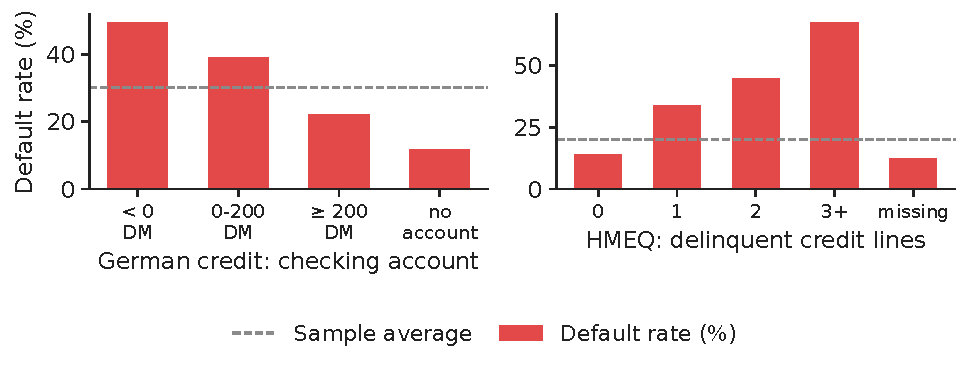
\includegraphics[width=\textwidth,height=0.445\textheight,keepaspectratio]{charts/en/default_rates.pdf}\end{center}\vspace{-3mm}
\chartsource{Source: UCI Statlog German credit; Baesens, Roesch and Scheule (2016), HMEQ. Data: 1,000 applicants (German credit); 5,960 loans (HMEQ).}
\vspace{0.5mm}
\begin{itemize}\setlength{\itemsep}{0pt}
  \item Probability of default (PD): 49.3\,\% with a negative checking balance, 11.7\,\% with no account
    \begin{itemize}\setlength{\itemsep}{0pt}
      \item 14.0\,\% with no delinquent line, 67.3\,\% with three or more.
    \end{itemize}
\end{itemize}
\par\vfill\manager{a model must at least reproduce these group rates on the validation set.}\par\vspace{0.5mm}
\par\vfill\noindent{\scriptsize\color{FooterGray}(own computation)}\hfill\qlink{NN\_L1\_default\_rates}{Quantlets/L1/NN_L1_default_rates}\par\vspace{0.5mm}
\end{frame}

\begin{frame}{Learning = minimising the average loss on training data, judged on new data}
\small
\intuition{we fit on one sample and pay for the errors on the next applicants.}
\[ \underbrace{\hat R_n(\btheta)=\frac1n\sum_{i=1}^n \ell\big(y_i,f(\vx_i;\btheta)\big)}_{\text{empirical risk (training)}}\qquad\text{vs.}\qquad \underbrace{R(\btheta)=\E_{(\vx,y)\sim P}\,\ell\big(y,f(\vx;\btheta)\big)}_{\text{risk on new applicants}} \]
{\footnotesize\begin{itemize}\setlength{\itemsep}{0pt}
  \item \textbf{\txtwhere}
    \begin{itemize}\setlength{\itemsep}{0pt}
      \item $P$ the unknown distribution of future applicants, $\ell$ the loss, $\hat R_n$ is minimised, $R$ is what the bank pays
    \end{itemize}
\end{itemize}\par}
\begin{itemize}\setlength{\itemsep}{2pt}
  \item Three sets: train (fit $\btheta$), validation (choose the model), test (report once).
  \item HMEQ, stratified: 3\,576 train, 1\,192 validation, 1\,192 test loans.
  \item No leakage: medians and scaling are fitted on the training part only.
\end{itemize}
\par\vfill\manager{the test set is used once, at the end (validation design: Lecture 3).}\par\vspace{0.5mm}
\par\vfill\noindent{\scriptsize\color{FooterGray}(Bishop \& Bishop, 2024, ch.~1)}\hfill\tryit{notebook \S2}\par\vspace{0.5mm}
\end{frame}


\section{Linear models are one-neuron networks}

\begin{frame}{Linear regression is one neuron with no activation}
\footnotesize
\intuition{a weighted sum of the inputs plus a bias; the squared loss is the Gaussian log-likelihood.}
\begin{columns}[T,onlytextwidth]
\begin{column}{0.53\textwidth}
\[ \hat y=\vw^\top\vx+b,\qquad \mathrm{MSE}(\vw,b)=\frac1n\sum_{i=1}^n\big(y_i-\vw^\top\vx_i-b\big)^2 \]
{\footnotesize\begin{itemize}\setlength{\itemsep}{0pt}
  \item \textbf{\txtwhere}
    \begin{itemize}\setlength{\itemsep}{0pt}
      \item $\vx\in\R^d$ the inputs, $\vw$ the weights, $b$ the bias
      \item Mean squared error (MSE) the loss
    \end{itemize}
\end{itemize}\par}\[ \varepsilon_i\iid\mathcal N(0,\sigma^2):\ \ -\log L=\tfrac{n}{2}\log 2\pi\sigma^2+\tfrac{n}{2\sigma^2}\mathrm{MSE} \]
\end{column}
\begin{column}{0.44\textwidth}
\begin{itemize}\setlength{\itemsep}{2pt}
  \item Maximum likelihood = least squares: the same $\hat\vw=(\mX^\top\mX)^{-1}\mX^\top\vy$.
  \item A network has no closed form: it is trained by gradient descent (Lecture 2).
  \item California housing, latitude only: held-out MSE 0.896 for the line.
\end{itemize}
\end{column}
\end{columns}
\par\vfill\manager{a linear fit is the benchmark every regression network must beat out of sample.}\par\vspace{0.5mm}
\par\vfill\noindent{\scriptsize\color{FooterGray}(Bishop \& Bishop, 2024, ch.~4)}\par\vspace{0.5mm}
\end{frame}

\begin{frame}{Logistic regression is one neuron with a sigmoid}
\footnotesize
\intuition{the neuron outputs a probability, and the loss is the Bernoulli negative log-likelihood (cross-entropy).}
\begin{columns}[T,onlytextwidth]
\begin{column}{0.53\textwidth}
\[ p_i=\sigma(\vw^\top\vx_i+b)=\frac{1}{1+e^{-z_i}},\qquad \nabla_{\vw}\loss=\frac1n\sum_{i=1}^n (p_i-y_i)\,\vx_i \]
\[ \loss(\vw,b)=-\frac1n\sum_{i=1}^n\big[y_i\log p_i+(1-y_i)\log(1-p_i)\big] \]
{\footnotesize\begin{itemize}\setlength{\itemsep}{0pt}
  \item \textbf{\txtwhere}
    \begin{itemize}\setlength{\itemsep}{0pt}
      \item $z_i$ the logit (log-odds), $\sigma$ the sigmoid, $y_i\in\{0,1\}$ default
      \item Derivation in the appendix
    \end{itemize}
\end{itemize}\par}
\end{column}
\begin{column}{0.44\textwidth}
\begin{itemize}\setlength{\itemsep}{2pt}
  \item The gradient is error times input: the same form will appear in every layer of backpropagation.
  \item $e^{w_j}$ is the odds ratio for a one-unit change of $x_j$.
  \item Convex loss: one global minimum.
\end{itemize}
\end{column}
\end{columns}
\par\vfill\manager{the logistic score is the industry standard for PD models.}\par\vspace{0.5mm}
\par\vfill\noindent{\scriptsize\color{FooterGray}(Bishop \& Bishop, 2024, ch.~5)}\par\vspace{0.5mm}
\end{frame}

\begin{frame}{Delinquencies and a missing debt ratio raise the odds of default most}
\small
\intuition{HMEQ, standardised inputs: each coefficient is the change in log-odds per one standard deviation.}
\begin{center}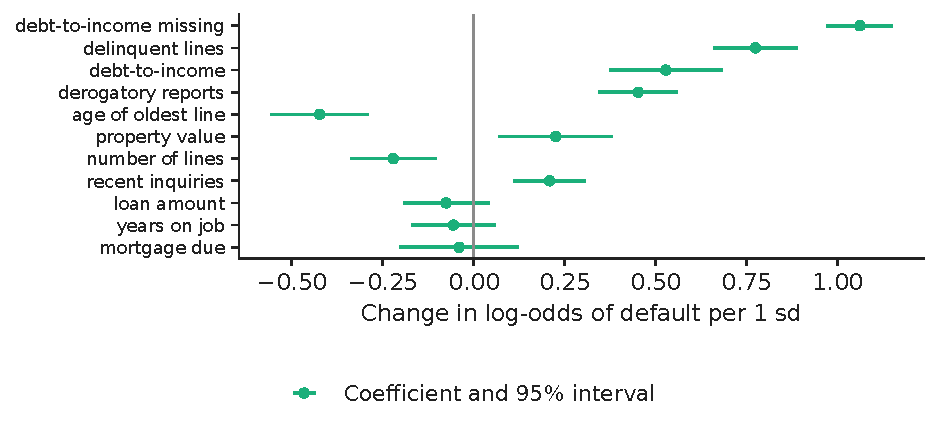
\includegraphics[width=\textwidth,height=0.417\textheight,keepaspectratio]{charts/en/logit_coef.pdf}\end{center}\vspace{-3mm}
\chartsource{Source: Baesens, Roesch and Scheule (2016), HMEQ data. Data: 3,576 training loans.}
\vspace{0.5mm}
\begin{itemize}\setlength{\itemsep}{0pt}
  \item Odds ratios $e^{w_j}$: 2.89 for a missing debt ratio, 2.17 for delinquent lines, 0.65 for an older credit history (McFadden pseudo-$R^2$ 0.374).
\end{itemize}
\par\vfill\manager{a sign against credit sense (property value) is a reason to inspect the data.}\par\vspace{0.5mm}
\par\vfill\noindent{\scriptsize\color{FooterGray}(own computation)}\hfill\qlink{NN\_L1\_logit\_coef}{Quantlets/L1/NN_L1_logit_coef}\par\vspace{0.5mm}
\end{frame}

\begin{frame}{The forward pass of one real applicant, step by step}
\small
\intuition{the score is a sum of contributions $w_jx_j$; the sigmoid turns it into a probability.}
\begin{columns}[T,onlytextwidth]
\begin{column}{0.50\textwidth}
{\footnotesize\renewcommand{\arraystretch}{1.05}\setlength{\tabcolsep}{4pt}
\begin{tabular}{@{}lrrr@{}}\toprule
Input & $x_j$ & $w_j$ & $w_jx_j$ \\ \midrule
delinquent credit lines & 1.46 & 0.774 & \ensuremath{+}1.13 \\
number of credit lines & 2.81 & \ensuremath{-}0.221 & \ensuremath{-}0.62 \\
debt-to-income missing & \ensuremath{-}0.51 & 1.062 & \ensuremath{-}0.54 \\
bias $b$ &  &  & \ensuremath{-}1.99 \\
8 other inputs &  &  & \ensuremath{+}0.31 \\
\textbf{score $z$} &  &  & \textbf{\ensuremath{-}1.71} \\
\bottomrule\end{tabular}}
\end{column}
\begin{column}{0.47\textwidth}
\begin{itemize}\setlength{\itemsep}{2pt}
  \item Applicant from the test set who later defaulted: loan 15\,400 USD, debt-to-income 36.4\,\%, 2 delinquent lines.
  \item Output: $p=\sigma(z)=$ 15.3\,\%, below the 50\,\% default cut-off.
  \item Inputs $x_j$ are standardised: $x_j=(\text{raw}_j-\bar x_j)/s_j$ with training means and standard deviations.
\end{itemize}
\end{column}
\end{columns}
\par\vfill\manager{the cut-off is a business choice: Section 5 sets it from the cost of a missed default.}\par\vspace{0.5mm}
\par\vfill\noindent{\scriptsize\color{FooterGray}(own computation)}\hfill\tryit{notebook \S2}\par\vspace{0.5mm}
\end{frame}

\begin{frame}{Missing values as predictors of default}
\small
\intuition{applicants who do not report their debt ratio default far more often: missingness is information.}
\[ \tilde x_{ij}=\begin{cases}x_{ij}&\text{observed}\\ \mathrm{med}_{\text{train}}(x_j)&\text{missing}\end{cases},\qquad m_{ij}=\mathbb 1\{x_{ij}\ \text{missing}\} \]
\begin{itemize}\setlength{\itemsep}{2pt}
  \item Debt-to-income is missing for 21.3\,\% of HMEQ loans.
  \item Default rate 62.0\,\% when it is missing against 8.6\,\% when it is reported.
  \item Each of the 10 numeric inputs gets a median fill and an indicator $m_{ij}$
    \begin{itemize}\setlength{\itemsep}{0pt}
      \item With 8 dummies for reason and job, the network sees $d=$ 28 inputs.
    \end{itemize}
\end{itemize}
\par\vfill\manager{never drop rows with missing values in credit data: you would drop the riskiest applicants.}\par\vspace{0.5mm}
\par\vfill\noindent{\scriptsize\color{FooterGray}(Baesens, Rösch \& Scheule, 2016)}\hfill\tryit{notebook \S2}\par\vspace{0.5mm}
\end{frame}


\section{The perceptron}

\begin{frame}{From a logical neuron to a learning machine}
\footnotesize
\intuition{McCulloch and Pitts wrote the neuron as a threshold unit; Rosenblatt made its weights learn from examples.}
\begin{columns}[T,onlytextwidth]
\begin{column}{0.53\textwidth}
\[ \hat y=\operatorname{step}(\vw^\top\vx+b)=\begin{cases}+1&\vw^\top\vx+b>0\\-1&\text{otherwise}\end{cases} \]
{\footnotesize\begin{itemize}\setlength{\itemsep}{0pt}
  \item \textbf{\txtwhere}
    \begin{itemize}\setlength{\itemsep}{0pt}
      \item $\vx$ the inputs (dendrites), $\vw$ the synaptic weights, $-b$ the firing threshold
      \item $\hat y$ the class (axon)
    \end{itemize}
\end{itemize}\par}
\end{column}
\begin{column}{0.44\textwidth}
\begin{itemize}\setlength{\itemsep}{2pt}
  \item 1943: logical calculus of threshold neurons (McCulloch \& Pitts, 1943).
  \item 1958: the perceptron learns $\vw$ from labelled examples (Rosenblatt, 1958).
  \item 1969: a single layer cannot represent XOR (Minsky \& Papert, 1969).
  \item 1986: backpropagation trains several layers (Rumelhart, Hinton \& Williams, 1986).
\end{itemize}
\end{column}
\end{columns}
\par\vfill\manager{the perceptron is a linear classifier: its boundary $\vw^\top\vx+b=0$ is a hyperplane.}\par\vspace{0.5mm}
\par\vfill\noindent{\scriptsize\color{FooterGray}(Bishop \& Bishop, 2024, ch.~5)}\par\vspace{0.5mm}
\end{frame}

\begin{frame}{The perceptron learns only from its mistakes}
\footnotesize
\intuition{when an example is misclassified, the weights move towards it; otherwise nothing changes.}
\begin{columns}[T,onlytextwidth]
\begin{column}{0.53\textwidth}
\[ \text{if}\ y_i(\vw^\top\vx_i+b)\le 0:\qquad \vw\leftarrow\vw+\eta\,y_i\vx_i,\quad b\leftarrow b+\eta\,y_i \]
\[ \loss_P(\vw,b)=-\!\!\sum_{i\in\mathcal M}\! y_i(\vw^\top\vx_i+b) \]
{\footnotesize\begin{itemize}\setlength{\itemsep}{0pt}
  \item \textbf{\txtwhere}
    \begin{itemize}\setlength{\itemsep}{0pt}
      \item $y_i\in\{-1,+1\}$, $\eta>0$ the learning rate, $\mathcal M$ the set of misclassified examples
      \item $\loss_P$ the perceptron criterion
    \end{itemize}
\end{itemize}\par}
\end{column}
\begin{column}{0.44\textwidth}
\begin{itemize}\setlength{\itemsep}{2pt}
  \item The update is one step of stochastic gradient descent (SGD) on $\loss_P$ for one misclassified example.
  \item Unlike logistic regression, correct examples give no gradient: the perceptron ignores how confident it is.
  \item No probability comes out: only a class.
\end{itemize}
\end{column}
\end{columns}
\par\vfill\manager{for credit, a class without a probability cannot be priced or set against a cost.}\par\vspace{0.5mm}
\par\vfill\noindent{\scriptsize\color{FooterGray}(Rosenblatt, 1958; Bishop \& Bishop, 2024, ch.~5)}\par\vspace{0.5mm}
\end{frame}

\begin{frame}{If the classes can be separated, the perceptron stops after finitely many mistakes}
\small
\intuition{a wide margin between the classes means few corrections are needed.}
\[ \exists\,\vw^*,\ \|\vw^*\|=1:\ y_i\,\vw^{*\top}\vx_i\ge\gamma>0\ \ \forall i,\quad \|\vx_i\|\le R\ \ \Longrightarrow\ \ \#\text{mistakes}\le\Big(\frac{R}{\gamma}\Big)^2 \]
{\footnotesize\begin{itemize}\setlength{\itemsep}{0pt}
  \item \textbf{\txtwhere}
    \begin{itemize}\setlength{\itemsep}{0pt}
      \item $\gamma$ the margin of the best separating hyperplane, $R$ the radius of the data, the bias is absorbed in $\vx$ (a constant 1)
    \end{itemize}
\end{itemize}\par}
\begin{itemize}\setlength{\itemsep}{2pt}
  \item Novikoff's theorem (1962): the bound does not depend on the number of examples or on the dimension.
  \item Proof idea: $\vw^\top\vw^*$ grows by at least $\gamma$ per mistake, $\|\vw\|^2$ by at most $R^2$ (appendix).
  \item If no separating hyperplane exists, the theorem says nothing and the weights cycle for ever.
\end{itemize}
\par\vfill\manager{real default data are never separable: applicants with the same file can repay or default.}\par\vspace{0.5mm}
\par\vfill\noindent{\scriptsize\color{FooterGray}(Novikoff, 1962)}\hfill\tryit{notebook \S3}\par\vspace{0.5mm}
\end{frame}

\begin{frame}{The perceptron does not converge on non-separable credit data}
\small
\intuition{the classes overlap, so every epoch corrects some loans and breaks others.}
\begin{center}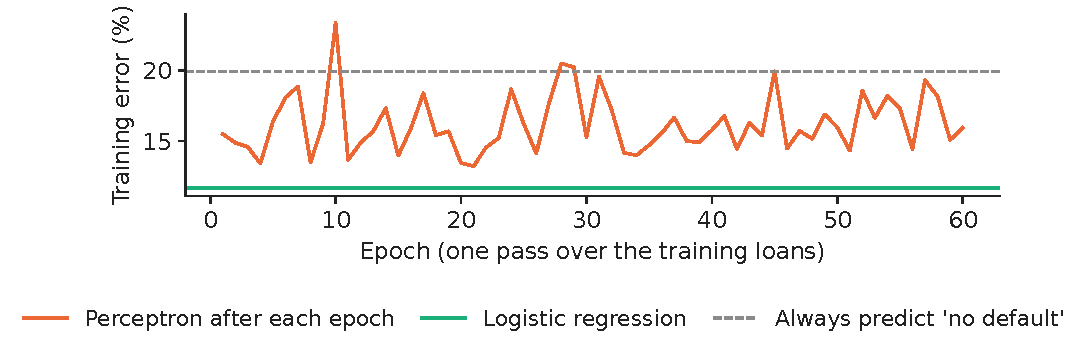
\includegraphics[width=\textwidth,height=0.469\textheight,keepaspectratio]{charts/en/perceptron_errors.pdf}\end{center}\vspace{-3mm}
\chartsource{Source: Baesens, Roesch and Scheule (2016), HMEQ data. Data: 3,576 training loans.}
\vspace{0.5mm}
\begin{itemize}\setlength{\itemsep}{0pt}
  \item Error after each of 60 epochs: 13.2--23.4\,\%, against 11.7\,\% for logistic regression and 19.9\,\% for `always no default'.
\end{itemize}
\par\vfill\manager{a smooth loss and a probability output fix this: networks use sigmoids, not steps.}\par\vspace{0.5mm}
\par\vfill\noindent{\scriptsize\color{FooterGray}(own computation)}\hfill\qlink{NN\_L1\_perceptron\_errors}{Quantlets/L1/NN_L1_perceptron_errors}\par\vspace{0.5mm}
\end{frame}

\begin{frame}{The XOR problem and the hidden layer}
\small
\intuition{XOR is true when exactly one input is on; the two positive points sit on a diagonal.}
\vspace{-1mm}\[ h_k=\tanh(\vw_k^\top\vx+b_k),\ k=1,2;\qquad p=\sigma(v_1h_1+v_2h_2+c) \]\vspace{-2mm}
\begin{center}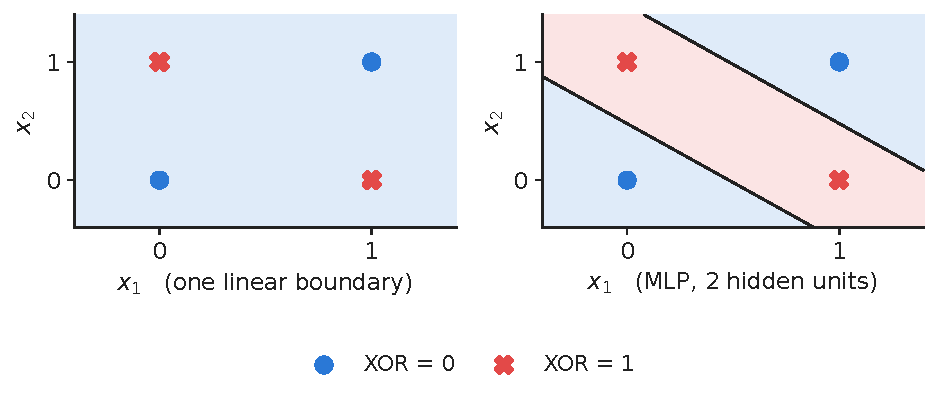
\includegraphics[width=\textwidth,height=0.419\textheight,keepaspectratio]{charts/en/xor.pdf}\end{center}\vspace{-3mm}
\chartsource{Source: logical XOR table (no data). Data: the four XOR inputs.}
\vspace{0.5mm}
\begin{itemize}\setlength{\itemsep}{0pt}
  \item Accuracy on the four points: 50\,\% for any linear boundary, 100\,\% with two hidden units.
\end{itemize}
\par\vfill\manager{interactions such as `high debt and short history' are XOR-like.}\par\vspace{0.5mm}
\par\vfill\noindent{\scriptsize\color{FooterGray}(Minsky \& Papert, 1969) \simlabel}\hfill\qlink{NN\_L1\_xor}{Quantlets/L1/NN_L1_xor}\par\vspace{0.5mm}
\end{frame}


\section{The multilayer perceptron}

\begin{frame}{An MLP alternates affine maps and nonlinear activations}
\small
\intuition{each layer computes new features from the previous ones; the last layer is a logistic regression on them.}
\[ \vh^{(0)}=\vx,\quad \vh^{(l)}=a\big(\mW^{(l)}\vh^{(l-1)}+\vb^{(l)}\big),\ l=1,\dots,L-1,\quad p(\vx)=\sigma\big(\vw^{(L)\top}\vh^{(L-1)}+b^{(L)}\big) \]
{\footnotesize\begin{itemize}\setlength{\itemsep}{0pt}
  \item \textbf{\txtwhere}
    \begin{itemize}\setlength{\itemsep}{0pt}
      \item $\mW^{(l)}\in\R^{H_l\times H_{l-1}}$, $\vb^{(l)}$ weights and biases of layer $l$, of width $H_l$ ($H_0=d$), $a$ the activation, element by element
    \end{itemize}
\end{itemize}\par}
\begin{itemize}\setlength{\itemsep}{2pt}
  \item Without $a$, the layers collapse: $\mW^{(2)}\mW^{(1)}\vx$ is again linear (appendix).
  \item Our credit network: $d=$ 28 inputs, two hidden layers of 64 rectified linear units (ReLU), one sigmoid output (`MLP 64-64').
\end{itemize}
\par\vfill\manager{width and depth are design choices
    \begin{itemize}\setlength{\itemsep}{0pt}
      \item Section 5 chooses them on the validation set.
    \end{itemize}}\par\vspace{0.5mm}
\par\vfill\noindent{\scriptsize\color{FooterGray}(Bishop \& Bishop, 2024, ch.~6)}\hfill\tryit{notebook \S4}\par\vspace{0.5mm}
\end{frame}

\begin{frame}{Activation functions: smooth, cheap, and with a usable gradient}
\small
\vspace{-1mm}\[ \sigma(z)=\tfrac{1}{1+e^{-z}},\ \ \tanh(z)=\tfrac{e^z-e^{-z}}{e^z+e^{-z}},\ \ \mathrm{ReLU}(z)=\max(0,z),\ \ \mathrm{GELU}(z)=z\,\Phi(z) \]\vspace{-2mm}
\begin{center}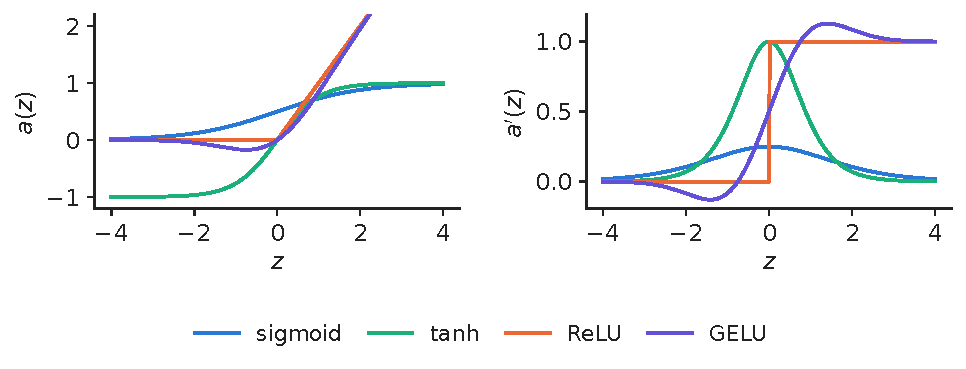
\includegraphics[width=\textwidth,height=0.316\textheight,keepaspectratio]{charts/en/activations.pdf}\end{center}\vspace{-3mm}
\chartsource{Source: analytic functions (no data). Data: functions plotted on [-4, 4].}
\vspace{0.5mm}
\begin{itemize}\setlength{\itemsep}{0pt}
  \item Sigmoid and tanh saturate ($\sigma'\le$ 0.25)
    \begin{itemize}\setlength{\itemsep}{0pt}
      \item The rectified linear unit (ReLU) passes gradient 1 for $z>0$
      \item The Gaussian error linear unit (GELU, $\Phi$ the normal distribution function) is used in transformers.
    \end{itemize}
\end{itemize}
\par\vfill\manager{use ReLU in hidden layers
    \begin{itemize}\setlength{\itemsep}{0pt}
      \item The output activation follows the target.
    \end{itemize}}\par\vspace{0.5mm}
\par\vfill\noindent{\scriptsize\color{FooterGray}(Bishop \& Bishop, 2024, ch.~6) \simlabel}\hfill\qlink{NN\_L1\_activations}{Quantlets/L1/NN_L1_activations}\par\vspace{0.5mm}
\end{frame}

\begin{frame}{The output layer and the loss come from the type of the target}
\small
\intuition{each pair (output activation, loss) is a maximum-likelihood estimator for one distribution of $y$.}
{\scriptsize\renewcommand{\arraystretch}{1.05}\setlength{\tabcolsep}{4pt}
\begin{tabular}{@{}p{0.20\textwidth}p{0.18\textwidth}p{0.30\textwidth}p{0.24\textwidth}@{}}\toprule
Target & Output & Loss & Example \\ \midrule
real number & $\hat y=z$ & MSE: $\frac1n\sum(y_i-\hat y_i)^2$ & house value, a price \\
binary & $p=\sigma(z)$ & cross-entropy: $-\frac1n\sum[y\log p+(1-y)\log(1-p)]$ & default, fraud \\
$K$ classes & $p_k=\frac{e^{z_k}}{\sum_j e^{z_j}}$ & $-\frac1n\sum_i\log p_{i,y_i}$ & rating grade, news sentiment \\
quantile $\tau$ & $\hat q=z$ & pinball: $\frac1n\sum\rho_\tau(y_i-\hat q_i)$ & value at risk (VaR), Lecture 2 \\
\bottomrule\end{tabular}}
\par\vspace{0.5mm}{\scriptsize \begin{itemize}\setlength{\itemsep}{0pt}
  \item $\rho_\tau(u)=u(\tau-\mathbb 1\{u<0\})$; softmax with $K=2$ reduces to the sigmoid.
\end{itemize}}
\par\vfill\manager{a PD model needs a sigmoid output and cross-entropy, so that its scores are probabilities.}\par\vspace{0.5mm}
\par\vfill\noindent{\scriptsize\color{FooterGray}(Bishop \& Bishop, 2024, ch.~5--6)}\par\vspace{0.5mm}
\end{frame}

\begin{frame}{A small MLP already has hundreds of times more parameters than the logistic score}
\small
\intuition{every connection is a weight, and every unit has a bias.}
\[ |\btheta|=\sum_{l=1}^{L}(H_{l-1}+1)\,H_l,\qquad H_0=d,\ H_L=1 \]
\begin{itemize}\setlength{\itemsep}{2pt}
  \item Logistic regression on HMEQ: $(d+1)\cdot1=$ 29 parameters.
  \item MLP 64-64: $(d+1)\cdot64+65\cdot64+65\cdot1=$ 6\,081 parameters for 3\,576 training loans.
  \item More parameters than training defaults: without validation-based stopping the network would memorise them (Lecture 3).
  \item Here every MLP is trained with Adam (Lecture 2) and keeps the weights of its best validation epoch.
\end{itemize}
\par\vfill\manager{count parameters before training: it tells you how much data and regularisation you will need.}\par\vspace{0.5mm}
\par\vfill\noindent{\scriptsize\color{FooterGray}}\hfill\tryit{notebook \S4}\par\vspace{0.5mm}
\end{frame}

\begin{frame}{One hidden layer can approximate any continuous function}
\small
\intuition{enough sigmoid `bumps', added together, can trace any smooth curve on a bounded domain.}
\[ \forall\,g\in C(K),\ \forall\,\varepsilon>0\ \ \exists\,H,\ v_k,\vw_k,b_k:\quad \sup_{\vx\in K}\Big|g(\vx)-\sum_{k=1}^{H}v_k\,\sigma(\vw_k^\top\vx+b_k)\Big|<\varepsilon \]
{\footnotesize\begin{itemize}\setlength{\itemsep}{0pt}
  \item \textbf{\txtwhere}
    \begin{itemize}\setlength{\itemsep}{0pt}
      \item $K\subset\R^d$ compact, $g$ continuous, $\sigma$ sigmoidal (Cybenko, 1989) or non-polynomial (Hornik, 1991)
    \end{itemize}
\end{itemize}\par}
\begin{itemize}\setlength{\itemsep}{2pt}
  \item What it says: the MLP family is rich enough.
  \item What it does not say: how large $H$ must be, whether gradient descent finds the weights, or whether they generalise.
\end{itemize}
\par\vfill\manager{the theorem justifies trying an MLP
    \begin{itemize}\setlength{\itemsep}{0pt}
      \item Only out-of-sample tests justify keeping it.
    \end{itemize}}\par\vspace{0.5mm}
\par\vfill\noindent{\scriptsize\color{FooterGray}(Cybenko, 1989; Hornik, 1991)}\par\vspace{0.5mm}
\end{frame}

\begin{frame}{More hidden units trace the price geography of California}
\small
\intuition{values peak near Los Angeles and San Francisco; $\hat y(x)=c+\sum_{k=1}^{H}v_k\sigma(w_kx+b_k)$ with $H=1,3,50$.}
\begin{center}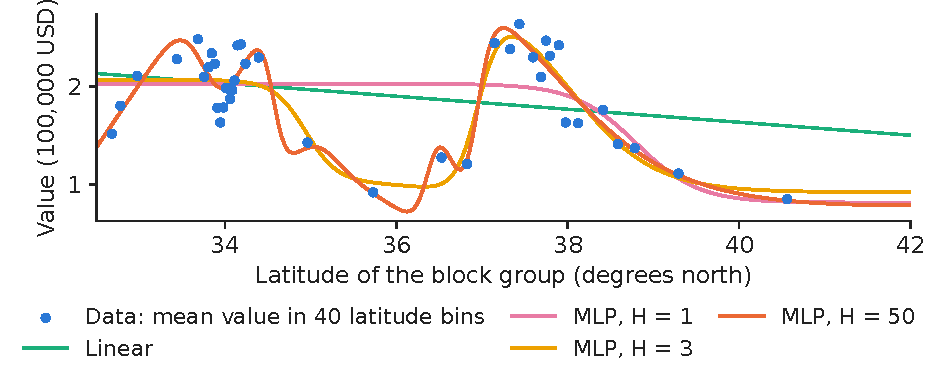
\includegraphics[width=\textwidth,height=0.412\textheight,keepaspectratio]{charts/en/uat_california.pdf}\end{center}\vspace{-3mm}
\chartsource{Source: StatLib, California housing, 1990 census (Pace and Barry, 1997). Data: 19,648 block groups below the source cap.}
\vspace{0.5mm}
\begin{itemize}\setlength{\itemsep}{0pt}
  \item Held-out MSE: linear 0.896, $H=1$ 0.855, $H=3$ 0.757, $H=50$ 0.731 (992 block groups at the 500,000 USD cap left out).
\end{itemize}
\par\vfill\manager{location effects are nonlinear: a linear term in latitude cannot price them.}\par\vspace{0.5mm}
\par\vfill\noindent{\scriptsize\color{FooterGray}(own computation)}\hfill\qlink{NN\_L1\_uat\_california}{Quantlets/L1/NN_L1_uat_california}\par\vspace{0.5mm}
\end{frame}

\begin{frame}{Depth and width of a network}
\small
\intuition{each layer composes the features of the previous one, so the number of linear pieces can grow with depth.}
\[ \text{ReLU MLP:}\ \ f(\vx)\ \text{is piecewise linear; number of linear regions up to}\ \ O\big(H^{dL}\big) \]
{\footnotesize\begin{itemize}\setlength{\itemsep}{0pt}
  \item \textbf{\txtwhere}
    \begin{itemize}\setlength{\itemsep}{0pt}
      \item $H$ the width of each layer, $L$ the number of hidden layers, $d$ the input dimension (bound of Montúfar et al., 2014)
    \end{itemize}
\end{itemize}\par}
\begin{itemize}\setlength{\itemsep}{2pt}
  \item For some functions a shallow net needs exponentially more units than a deep one.
  \item On tabular credit data, two or three hidden layers are usually enough
    \begin{itemize}\setlength{\itemsep}{0pt}
      \item Depth pays off on images, text and sequences.
    \end{itemize}
\end{itemize}
\par\vfill\manager{start with 2 hidden layers on tabular data
    \begin{itemize}\setlength{\itemsep}{0pt}
      \item Go deeper only if validation loss keeps falling.
    \end{itemize}}\par\vspace{0.5mm}
\par\vfill\noindent{\scriptsize\color{FooterGray}(Bishop \& Bishop, 2024, ch.~6)}\par\vspace{0.5mm}
\end{frame}

\begin{frame}{An MLP bends the decision boundary, but two inputs carry little extra signal}
\small
\intuition{predicted PD for two HMEQ variables: straight bands for the logistic model, curved regions for the MLP.}
\begin{center}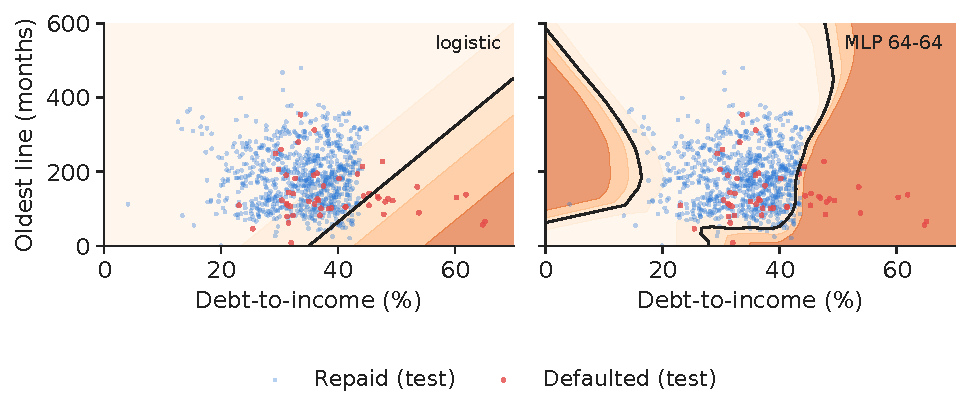
\includegraphics[width=\textwidth,height=0.434\textheight,keepaspectratio]{charts/en/boundary_hmeq.pdf}\end{center}\vspace{-3mm}
\chartsource{Source: Baesens, Roesch and Scheule (2016), HMEQ data. Data: 2,708 training and 871 test loans with both variables.}
\vspace{0.5mm}
\begin{itemize}\setlength{\itemsep}{0pt}
  \item Area under the receiver operating characteristic (ROC) curve (AUC) = $\Pr(p_{\text{default}}>p_{\text{good}})$
    \begin{itemize}\setlength{\itemsep}{0pt}
      \item With these two inputs: logistic 0.744, MLP 64-64 0.736.
    \end{itemize}
\end{itemize}
\par\vfill\manager{a flexible boundary pays only if the inputs carry the signal.}\par\vspace{0.5mm}
\par\vfill\noindent{\scriptsize\color{FooterGray}(own computation)}\hfill\qlink{NN\_L1\_boundary\_hmeq}{Quantlets/L1/NN_L1_boundary_hmeq}\par\vspace{0.5mm}
\end{frame}


\section{Case study: credit scoring with real loans}

\begin{frame}{The protocol: same split, same inputs, three models}
\small
\intuition{a fair comparison changes only the model; data, split and metric stay fixed before anything is trained.}
\begin{columns}[T,onlytextwidth]
\begin{column}{0.50\textwidth}
\begin{itemize}\setlength{\itemsep}{2pt}
  \item Logistic regression: maximum likelihood, no penalty on HMEQ
    \begin{itemize}\setlength{\itemsep}{0pt}
      \item A mild ridge penalty ($C=1$) on German credit.
    \end{itemize}
  \item MLP: ReLU layers, Adam with learning rate $10^{-3}$, batches of 128 (64 on German credit), best validation epoch, 5 seeds.
  \item Extreme gradient boosting (XGBoost): depth 4, learning rate 0.03, early stopping on validation (Chen \& Guestrin, 2016).
\end{itemize}
\end{column}
\begin{column}{0.47\textwidth}
\begin{itemize}\setlength{\itemsep}{2pt}
  \item HMEQ: one stratified 60/20/20 split
    \begin{itemize}\setlength{\itemsep}{0pt}
      \item AUC, ROC curve, calibration, bootstrap interval of the AUC gain.
    \end{itemize}
  \item German credit: 5 times repeated 5-fold cross-validation (25 test folds), corrected $t$-test.
  \item Seed 20261108 (+ run index)
    \begin{itemize}\setlength{\itemsep}{0pt}
      \item Trained on the central processing unit (CPU), under a minute per model family.
    \end{itemize}
\end{itemize}
\end{column}
\end{columns}
\par\vfill\manager{write the protocol down before training: it is what a model validator will ask for first.}\par\vspace{0.5mm}
\par\vfill\noindent{\scriptsize\color{FooterGray}}\hfill\tryit{notebook \S5}\par\vspace{0.5mm}
\end{frame}

\begin{frame}{On HMEQ, a wider hidden layer raises the test AUC above the logistic score}
\small
\intuition{one hidden layer of width $H$; each point is the mean of 5 seeds, the band their range.}
\begin{center}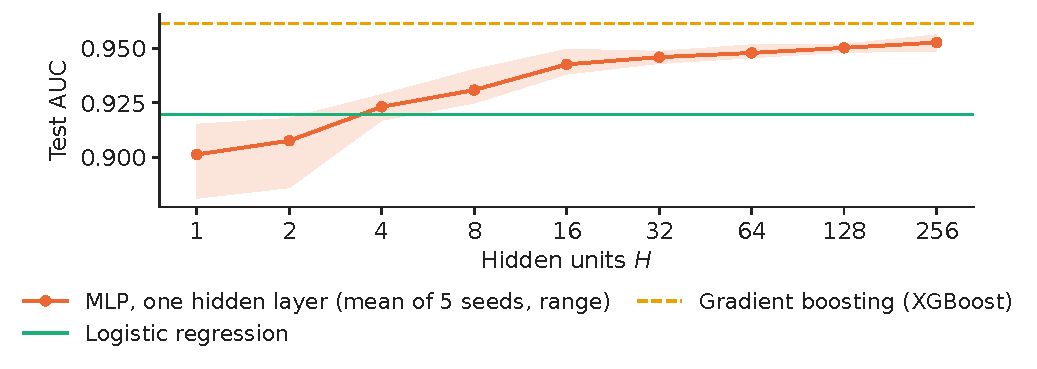
\includegraphics[width=\textwidth,height=0.440\textheight,keepaspectratio]{charts/en/width_auc.pdf}\end{center}\vspace{-3mm}
\chartsource{Source: Baesens, Roesch and Scheule (2016), HMEQ data. Data: 3,576 training, 1,192 validation, 1,192 test loans.}
\vspace{0.5mm}
\begin{itemize}\setlength{\itemsep}{0pt}
  \item AUC 0.901 at $H=1$, 0.953 at $H=$ 256
    \begin{itemize}\setlength{\itemsep}{0pt}
      \item Logistic 0.920, XGBoost 0.961
      \item The gain flattens after about 16 units.
    \end{itemize}
\end{itemize}
\par\vfill\manager{interactions matter here: the network beats the linear score, boosting beats both.}\par\vspace{0.5mm}
\par\vfill\noindent{\scriptsize\color{FooterGray}(own computation)}\hfill\qlink{NN\_L1\_width\_auc}{Quantlets/L1/NN_L1_width_auc}\par\vspace{0.5mm}
\end{frame}

\begin{frame}{At a 10\,\% false-alarm rate, the MLP catches more defaults than the logistic score}
\small
\intuition{the ROC curve plots $\Pr(p\ge c\mid\text{default})$ against $\Pr(p\ge c\mid\text{good})$ for every cut-off $c$.}
\begin{center}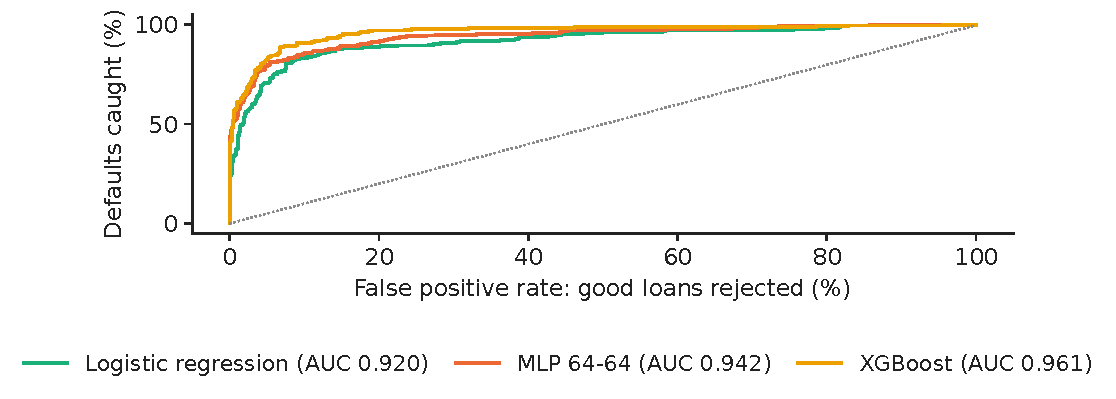
\includegraphics[width=\textwidth,height=0.396\textheight,keepaspectratio]{charts/en/roc_hmeq.pdf}\end{center}\vspace{-3mm}
\chartsource{Source: Baesens, Roesch and Scheule (2016), HMEQ data. Data: 1,192 test loans (238 defaults).}
\vspace{0.5mm}
\begin{itemize}\setlength{\itemsep}{0pt}
  \item Defaults caught when 10\,\% of good loans are rejected: logistic 83.2\,\%, MLP 85.3\,\%, XGBoost 90.8\,\% (238 test defaults).
\end{itemize}
\par\vfill\manager{read the curve at the rejection rate the business accepts, not only its area.}\par\vspace{0.5mm}
\par\vfill\noindent{\scriptsize\color{FooterGray}(own computation)}\hfill\qlink{NN\_L1\_roc\_hmeq}{Quantlets/L1/NN_L1_roc_hmeq}\par\vspace{0.5mm}
\end{frame}

\begin{frame}{The MLP gain on HMEQ is larger than seed noise and test-set noise}
\small
\intuition{one run proves nothing: we repeat the training and resample the test set.}
\[ \Delta=\mathrm{AUC}_{\mathrm{MLP}}-\mathrm{AUC}_{\text{logit}},\qquad \Delta^{*}_b=\mathrm{AUC}_{\mathrm{MLP}}(\mathcal T^*_b)-\mathrm{AUC}_{\text{logit}}(\mathcal T^*_b),\ b=1,\dots,2000 \]
{\footnotesize\begin{itemize}\setlength{\itemsep}{0pt}
  \item \textbf{\txtwhere}
    \begin{itemize}\setlength{\itemsep}{0pt}
      \item $\mathcal T^*_b$ a bootstrap resample of the 1\,192 test loans, the same resample for both models (paired)
    \end{itemize}
\end{itemize}\par}
\begin{itemize}\setlength{\itemsep}{2pt}
  \item Seeds: MLP 64-64 test AUC 0.945 on average over 5 seeds (standard deviation 0.004; range 0.942--0.951).
  \item Test noise: $\Delta=$ 0.023, 95\,\% bootstrap interval [0.008; 0.037]: zero is excluded.
  \item The seed spread of the logistic model is zero: its loss is convex.
\end{itemize}
\par\vfill\manager{report a model gain with an interval
    \begin{itemize}\setlength{\itemsep}{0pt}
      \item A gain inside the seed spread is not a gain.
    \end{itemize}}\par\vspace{0.5mm}
\par\vfill\noindent{\scriptsize\color{FooterGray}(own computation)}\hfill\tryit{notebook \S5}\par\vspace{0.5mm}
\end{frame}

\begin{frame}{The scores are close to calibrated probabilities}
\small
\intuition{in each decile of predicted PD, the observed default rate should equal the predicted one.}
\begin{center}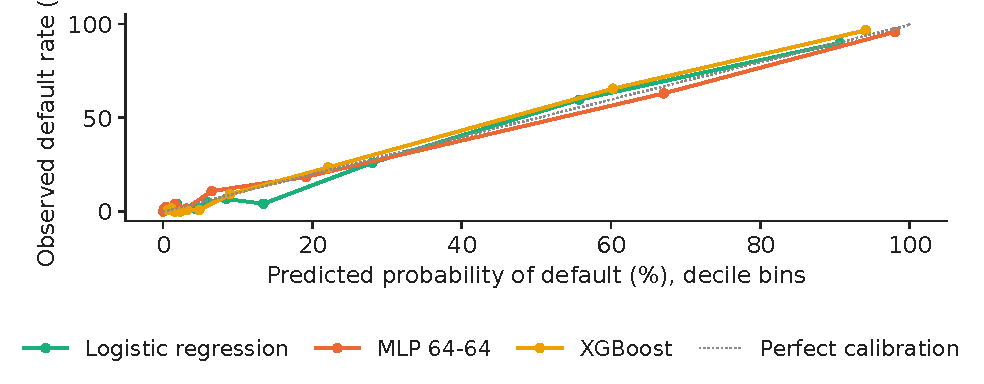
\includegraphics[width=\textwidth,height=0.441\textheight,keepaspectratio]{charts/en/calibration.pdf}\end{center}\vspace{-3mm}
\chartsource{Source: Baesens, Roesch and Scheule (2016), HMEQ data. Data: 1,192 test loans.}
\vspace{0.5mm}
\begin{itemize}\setlength{\itemsep}{0pt}
  \item Brier score $\frac1n\sum(p_i-y_i)^2$: logistic 0.0742, MLP 0.0625, XGBoost 0.0549
    \begin{itemize}\setlength{\itemsep}{0pt}
      \item Constant rate 0.1598.
    \end{itemize}
\end{itemize}
\par\vfill\manager{provisions and prices use the PD itself: check calibration, not only ranking.}\par\vspace{0.5mm}
\par\vfill\noindent{\scriptsize\color{FooterGray}(own computation)}\hfill\qlink{NN\_L1\_calibration}{Quantlets/L1/NN_L1_calibration}\par\vspace{0.5mm}
\end{frame}

\begin{frame}{On 1,000 German applicants, the MLP does not beat logistic regression}
\small
\intuition{each dot is the AUC of one held-out fold; the black bar is the mean of the 25 folds.}
\begin{center}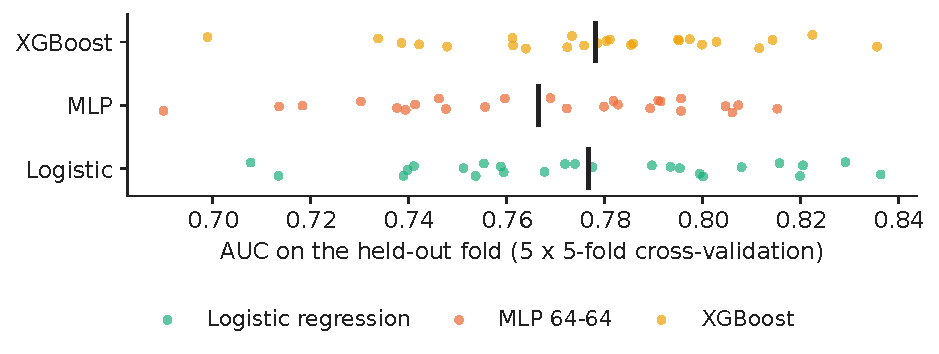
\includegraphics[width=\textwidth,height=0.482\textheight,keepaspectratio]{charts/en/german_cv.pdf}\end{center}\vspace{-3mm}
\chartsource{Source: UCI Machine Learning Repository, Statlog German credit. Data: 1,000 applicants, 25 held-out folds.}
\vspace{0.5mm}
\begin{itemize}\setlength{\itemsep}{0pt}
  \item Mean AUC: logistic 0.777, MLP 0.766, XGBoost 0.778
    \begin{itemize}\setlength{\itemsep}{0pt}
      \item MLP minus logistic: $t=$ \ensuremath{-}0.93, $p=$ 0.362 (next frame).
    \end{itemize}
\end{itemize}
\par\vfill\manager{with 1,000 rows, keep the logistic scorecard: the network adds risk, not accuracy.}\par\vspace{0.5mm}
\par\vfill\noindent{\scriptsize\color{FooterGray}(own computation)}\hfill\qlink{NN\_L1\_german\_cv}{Quantlets/L1/NN_L1_german_cv}\par\vspace{0.5mm}
\end{frame}

\begin{frame}{Why the usual $t$-test overstates differences in cross-validation}
\small
\intuition{the training sets of different folds overlap, so the fold scores are positively correlated.}
\[ t=\frac{\bar d}{\sqrt{\big(\frac{1}{J}+\frac{n_{\text{test}}}{n_{\text{train}}}\big)\,s_d^2}}\ \sim\ t_{J-1},\qquad d_j=\mathrm{AUC}^{\mathrm{MLP}}_j-\mathrm{AUC}^{\text{logit}}_j \]
{\footnotesize\begin{itemize}\setlength{\itemsep}{0pt}
  \item \textbf{\txtwhere}
    \begin{itemize}\setlength{\itemsep}{0pt}
      \item $J=$ 25 folds, $s_d^2$ the sample variance of $d_j$, $n_{\text{test}}/n_{\text{train}}=1/4$ for 5 folds
    \end{itemize}
\end{itemize}\par}
\begin{itemize}\setlength{\itemsep}{2pt}
  \item The term $n_{\text{test}}/n_{\text{train}}$ is the Nadeau--Bengio correction: without it, $t$ is far too large.
  \item MLP vs logistic: $t=$ \ensuremath{-}0.93 ($p=$ 0.362)
    \begin{itemize}\setlength{\itemsep}{0pt}
      \item XGBoost vs logistic: $t=$ 0.12 ($p=$ 0.909).
    \end{itemize}
\end{itemize}
\par\vfill\manager{a model change in a bank needs evidence that survives this correction.}\par\vspace{0.5mm}
\par\vfill\noindent{\scriptsize\color{FooterGray}(Nadeau \& Bengio, 2003)}\hfill\tryit{notebook \S6}\par\vspace{0.5mm}
\end{frame}

\begin{frame}{A missed default costs five times a rejected good applicant: cut at 1/6, not 1/2}
\small
\vspace{-1mm}\[ \text{reject if}\ \ c_{\mathrm{FN}}\,p\ \ge\ c_{\mathrm{FP}}(1-p)\iff p\ \ge\ \frac{c_{\mathrm{FP}}}{c_{\mathrm{FP}}+c_{\mathrm{FN}}}=\frac16 \]\vspace{-2mm}
\begin{center}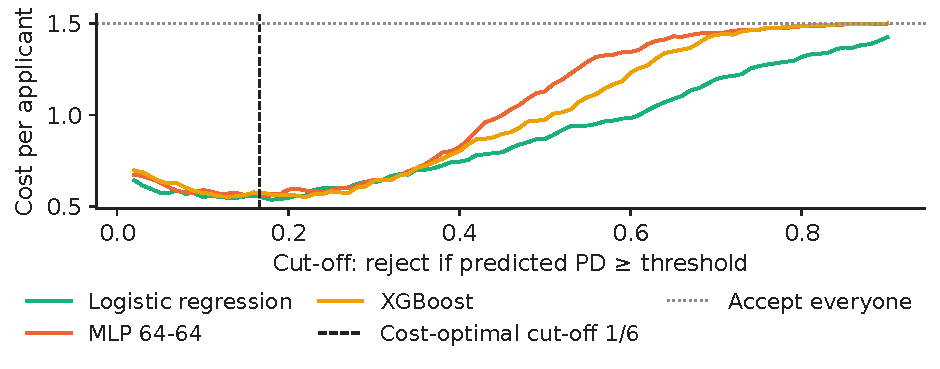
\includegraphics[width=\textwidth,height=0.396\textheight,keepaspectratio]{charts/en/cost_threshold.pdf}\end{center}\vspace{-3mm}
\chartsource{Source: UCI Machine Learning Repository, Statlog German credit. Data: 1,000 applicants, out-of-fold predictions.}
\vspace{0.5mm}
\begin{itemize}\setlength{\itemsep}{0pt}
  \item Cost per applicant (UCI cost matrix 5:1): at 1/6 logistic 0.554, MLP 0.568
    \begin{itemize}\setlength{\itemsep}{0pt}
      \item At 1/2 0.870 and 1.130
      \item Accept all 1.50.
    \end{itemize}
\end{itemize}
\par\vfill\manager{here the choice of cut-off matters more than the choice of model.}\par\vspace{0.5mm}
\par\vfill\noindent{\scriptsize\color{FooterGray}(own computation)}\hfill\qlink{NN\_L1\_cost\_threshold}{Quantlets/L1/NN_L1_cost_threshold}\par\vspace{0.5mm}
\end{frame}

\begin{frame}{A minimal MLP in PyTorch: about fifteen lines}
\small
\begin{columns}[T,onlytextwidth]
\begin{column}{0.55\textwidth}
{\ttfamily\scriptsize\setlength{\parindent}{0pt}import torch, torch.nn as nn\\
model = nn.Sequential(\\
~~~~nn.Linear(d, 64), nn.ReLU(),\\
~~~~nn.Linear(64, 64), nn.ReLU(),\\
~~~~nn.Linear(64, 1))~~~~~~~~~~~~\# logit z\\
loss\_fn = nn.BCEWithLogitsLoss()~~\# sigmoid + cross-entropy\\
opt = torch.optim.Adam(model.parameters(), lr=1e-3)\\
for epoch in range(300):\\
~~~~for xb, yb in train\_batches:\\
~~~~~~~~opt.zero\_grad()\\
~~~~~~~~loss = loss\_fn(model(xb), yb)\\
~~~~~~~~loss.backward()~~~~~~~~~~ \# backpropagation\\
~~~~~~~~opt.step()~~~~~~~~~~~~~~~~\# Adam update\\
~~~~\# evaluate on validation, keep the best weights\\
p = torch.sigmoid(model(x\_test))~~ \# predicted PD\par}
\end{column}
\begin{column}{0.42\textwidth}
\begin{itemize}\setlength{\itemsep}{2pt}
  \item \texttt{BCEWithLogitsLoss} combines the sigmoid and the cross-entropy in one numerically stable function.
  \item \texttt{backward()} computes all gradients by backpropagation
    \begin{itemize}\setlength{\itemsep}{0pt}
      \item \texttt{step()} applies the optimiser: both are Lecture 2.
    \end{itemize}
  \item The notebook adds the data pipeline, the validation stopping and the seeds.
\end{itemize}
\end{column}
\end{columns}
\par\vfill\manager{the same fifteen lines train every tabular network of this course
    \begin{itemize}\setlength{\itemsep}{0pt}
      \item Only data and layers change.
    \end{itemize}}\par\vspace{0.5mm}
\par\vfill\noindent{\scriptsize\color{FooterGray}(Paszke et al., 2019)}\hfill\tryit{notebook \S7}\par\vspace{0.5mm}
\end{frame}

\begin{frame}{When to use an MLP for tabular business data}
\small
\begin{columns}[T,onlytextwidth]
\begin{column}{0.49\textwidth}
\begin{block}{Evidence from this lecture}
\begin{itemize}\setlength{\itemsep}{2pt}
  \item HMEQ, 3\,576 loans: MLP AUC 0.945 vs logistic 0.920
    \begin{itemize}\setlength{\itemsep}{0pt}
      \item XGBoost 0.961.
    \end{itemize}
  \item German credit, 1,000 applicants: no significant difference ($p=$ 0.362).
  \item Both: the cut-off from the cost matrix matters more than the model.
\end{itemize}
\end{block}
\end{column}
\begin{column}{0.49\textwidth}
\begin{exampleblock}{Rule of thumb}
\begin{itemize}\setlength{\itemsep}{2pt}
  \item Few rows, engineered features, explanation required: logistic scorecard.
  \item Thousands of rows, interactions: test boosting and an MLP against it.
  \item Raw text, images, sequences, graphs, or a network shared across tasks: deep learning.
\end{itemize}
\end{exampleblock}
\end{column}
\end{columns}
\par\vfill\manager{choose the simplest model whose out-of-sample gain survives seeds, resampling and the cost matrix.}\par\vspace{0.5mm}
\end{frame}


\section{Wrap-up}

\begin{frame}{Key takeaways}
\small
\begin{itemize}\setlength{\itemsep}{4pt}
  \item Linear and logistic regression are one-neuron networks
    \begin{itemize}\setlength{\itemsep}{0pt}
      \item Their losses are likelihoods, their gradients are error times input.
    \end{itemize}
  \item The perceptron converges only on separable data
    \begin{itemize}\setlength{\itemsep}{0pt}
      \item Real credit data are not separable, and XOR shows the limit of one layer.
    \end{itemize}
  \item An MLP stacks affine maps and activations
    \begin{itemize}\setlength{\itemsep}{0pt}
      \item One hidden layer approximates any continuous function, depth makes it efficient.
    \end{itemize}
  \item On real loans: the MLP beats logistic regression on HMEQ (AUC 0.945 vs 0.920), not on German credit
    \begin{itemize}\setlength{\itemsep}{0pt}
      \item Boosting is the bar to clear.
    \end{itemize}
  \item Evaluate with seeds, intervals, calibration and the cost of errors, never with one accuracy number.
\end{itemize}
\end{frame}

\begin{frame}{Key equations}
\small
\begin{columns}[T,onlytextwidth]
\begin{column}{0.49\textwidth}
\[ p=\sigma(\vw^\top\vx+b) \]
\[ \loss=-\tfrac1n\textstyle\sum[y\log p+(1-y)\log(1-p)] \]
\[ \nabla_{\vw}\loss=\tfrac1n\textstyle\sum(p_i-y_i)\vx_i \]
\[ \vw\leftarrow\vw+\eta\,y_i\vx_i\ \ \text{if misclassified} \]
\end{column}
\begin{column}{0.49\textwidth}
\[ \vh^{(l)}=a\big(\mW^{(l)}\vh^{(l-1)}+\vb^{(l)}\big) \]
\[ |\btheta|=\textstyle\sum_l(H_{l-1}+1)H_l \]
\[ \#\text{mistakes}\le(R/\gamma)^2 \]
\[ \text{reject if}\ p\ge\frac{c_{\mathrm{FP}}}{c_{\mathrm{FP}}+c_{\mathrm{FN}}} \]
\end{column}
\end{columns}
\end{frame}

\begin{frame}{Research from our group: deep learning for business decisions}
\footnotesize
\begin{itemize}\setlength{\itemsep}{2pt}
  \item \textbf{Explainable fraud detection} (Diaconu \& Pele, 2026): compared XGBoost and CatBoost with a graph neural network (GNN), graph sample and aggregate (GraphSAGE), on the Institute of Electrical and Electronics Engineers, Computational Intelligence Society (IEEE-CIS) fraud data
    \begin{itemize}\setlength{\itemsep}{0pt}
      \item Boosting had the higher AUC, the graph model captured relational fraud patterns
      \item A multi-level explainable artificial intelligence (XAI) framework joins Shapley additive explanations (SHAP) with node and edge ablation --- replicated in Case study 1 (course site).
    \end{itemize}
  \item \textbf{Early warning of crypto `zombies'} (Będowska-Sójka, Wójcik \& Pele, 2026): machine-learning early warning of crypto-assets that become `zombie' assets --- Lecture 3.
  \item \textbf{Risk measures from language models} (Pele et al., 2026): value at risk (VaR) and expected shortfall (ES) obtained by prompting large language models (LLM) --- Lecture 12.
  \item \textbf{Foundation models for tail risk} (Jheng, Tak, Găman, Mazurencu-Marinescu-Pele \& Pele, 2026): zero-shot VaR and ES with conformal calibration in Central and Eastern European markets --- Lecture 13.
  \item \textbf{Seeing market anomalies} (Jheng, Pele, Tak \& Găman, 2026; best paper award at the International Conference on Business Excellence (ICBE) 2026): market indicators drawn as images and classified by a vision-language model (VLM), with natural-language rationales, tested out of sample on the S\&P 500 --- Lecture 14.
\end{itemize}
\par\vspace{0.5mm}{\scriptsize \begin{itemize}\setlength{\itemsep}{0pt}
  \item Findings as stated in the papers; numbers on the other slides come from our own computations.
\end{itemize}}
\end{frame}

\begin{frame}{Want to learn more?}
\small
\begin{columns}[T,onlytextwidth]
\begin{column}{0.52\textwidth}
\begin{itemize}\setlength{\itemsep}{4pt}
  \item \textbf{Bishop \& Bishop (2024)}, chapters 4--6: linear models, classification, deep networks: \href{https://www.bishopbook.com}{bishopbook.com}.
  \item \textbf{Dive into Deep Learning}, chapters 3--5, with PyTorch code: \href{https://d2l.ai}{d2l.ai}.
  \item \textbf{Goodfellow, Bengio \& Courville}, chapter 6: \href{https://www.deeplearningbook.org}{deeplearningbook.org}.
\end{itemize}
\end{column}
\begin{column}{0.45\textwidth}
\begin{itemize}\setlength{\itemsep}{4pt}
  \item \textbf{PyTorch tutorials}: \href{https://pytorch.org/tutorials}{pytorch.org/tutorials}.
  \item \textbf{This course}: code, data, notebooks, Quantlets --- \href{https://github.com/danpele/NEURAL_BIZ}{github.com/danpele/NEURAL\_BIZ}.
  \item \textbf{Credit scoring in depth}: Baesens, Rösch \& Scheule (2016).
\end{itemize}
\end{column}
\end{columns}
\end{frame}

\begin{frame}{Quiz 1: logistic regression as a neuron}
\small
\begin{itemize}
  \item Which loss makes a one-neuron network with a sigmoid output equal to logistic regression?
\end{itemize}
\vspace{2mm}
\begin{exampleblock}{Answer}
\begin{itemize}
  \item The cross-entropy, i.e.\ the Bernoulli negative log-likelihood
    \begin{itemize}\setlength{\itemsep}{0pt}
      \item Its gradient is $\frac1n\sum(p_i-y_i)\vx_i$.
    \end{itemize}
\end{itemize}
\end{exampleblock}
\end{frame}

\begin{frame}{Quiz 2: the perceptron on real data}
\small
\begin{itemize}
  \item Why does the training error of the perceptron on HMEQ jump between 13.2\,\% and 23.4\,\%?
\end{itemize}
\vspace{2mm}
\begin{exampleblock}{Answer}
\begin{itemize}
  \item The classes are not linearly separable, so Novikoff's bound does not apply: each correction of one loan breaks others.
\end{itemize}
\end{exampleblock}
\end{frame}

\begin{frame}{Quiz 3: counting parameters}
\small
\begin{itemize}
  \item How many parameters has an MLP on the HMEQ inputs ($d=$ 28) with one hidden layer of 32 units and one output?
\end{itemize}
\vspace{2mm}
\begin{exampleblock}{Answer}
\begin{itemize}
  \item $(d+1)\cdot32+(32+1)\cdot1=$ 961.
\end{itemize}
\end{exampleblock}
\end{frame}

\begin{frame}{Quiz 4: the cost-optimal cut-off}
\small
\begin{itemize}
  \item A missed default costs 5, a rejected good applicant costs 1.
    \begin{itemize}\setlength{\itemsep}{0pt}
      \item Above which PD should the bank reject?
    \end{itemize}
\end{itemize}
\vspace{2mm}
\begin{exampleblock}{Answer}
\begin{itemize}
  \item $p\ge c_{\mathrm{FP}}/(c_{\mathrm{FP}}+c_{\mathrm{FN}})=1/6$
    \begin{itemize}\setlength{\itemsep}{0pt}
      \item On German credit this cut-off lowers the logistic cost per applicant from 0.870 (cut-off 1/2) to 0.554.
    \end{itemize}
\end{itemize}
\end{exampleblock}
\end{frame}

\begin{frame}{Quiz 5: when is an MLP worth it?}
\small
\begin{itemize}
  \item On German credit the MLP has mean AUC 0.766 and logistic regression 0.777.
    \begin{itemize}\setlength{\itemsep}{0pt}
      \item What do you recommend?
    \end{itemize}
\end{itemize}
\vspace{2mm}
\begin{exampleblock}{Answer}
\begin{itemize}
  \item Keep the logistic scorecard: the difference is not significant ($p=$ 0.362) and the simpler model is easier to explain and validate.
\end{itemize}
\end{exampleblock}
\end{frame}

\begin{frame}{References (1/2)}
\scriptsize
\begin{itemize}\setlength{\itemsep}{0pt}\scriptsize
\item Bishop, C.\,M.\ \& Bishop, H.\ (2024). \textit{Deep Learning: Foundations and Concepts}. Springer. \href{https://doi.org/10.1007/978-3-031-45468-4}{doi:10.1007/978-3-031-45468-4}
\item Baesens, B., Rösch, D.\ \& Scheule, H.\ (2016). \textit{Credit Risk Analytics}. Wiley. \href{https://doi.org/10.1002/9781119449560}{doi:10.1002/9781119449560}
\item Będowska-Sójka, B., Wójcik, P.\ \& Pele, D.\,T.\ (2026). Early warning systems for cryptocurrency markets: Predicting `zombie' assets using machine learning. \textit{The North American Journal of Economics and Finance}, 81, 102543. \href{https://doi.org/10.1016/j.najef.2025.102543}{doi:10.1016/j.najef.2025.102543}
\item Chen, T.\ \& Guestrin, C.\ (2016). XGBoost: A scalable tree boosting system. \textit{Proceedings of KDD 2016}, 785--794. \href{https://doi.org/10.1145/2939672.2939785}{doi:10.1145/2939672.2939785}
\item Cybenko, G.\ (1989). Approximation by superpositions of a sigmoidal function. \textit{Mathematics of Control, Signals and Systems}, 2(4), 303--314. \href{https://doi.org/10.1007/BF02551274}{doi:10.1007/BF02551274}
\item Diaconu, D.\ \& Pele, D.\,T.\ (2026). Explainable AI in financial fraud detection: Evidence from the IEEE-CIS fraud dataset. \textit{Proceedings of the International Conference on Business Excellence}, 20(1), 118--132. \href{https://doi.org/10.2478/picbe-2026-0015}{doi:10.2478/picbe-2026-0015}
\item Grinsztajn, L., Oyallon, E.\ \& Varoquaux, G.\ (2022). Why do tree-based models still outperform deep learning on typical tabular data? \textit{Advances in Neural Information Processing Systems}, 35. \href{https://arxiv.org/abs/2207.08815}{arXiv:2207.08815}
\item Hofmann, H.\ (1994). Statlog (German Credit Data). UCI Machine Learning Repository. \href{https://doi.org/10.24432/C5NC77}{doi:10.24432/C5NC77}
\item Hornik, K.\ (1991). Approximation capabilities of multilayer feedforward networks. \textit{Neural Networks}, 4(2), 251--257. \href{https://doi.org/10.1016/0893-6080(91)90009-T}{doi:10.1016/0893-6080(91)90009-T}
\item Jheng, S.-L., Pele, D.\,T., Tak, R.\ \& Găman, Ș.\ (2026). A multimodal vision-language framework for financial anomaly detection. \textit{Proceedings of the International Conference on Business Excellence}, 20(1), 191--201. \href{https://doi.org/10.2478/picbe-2026-0020}{doi:10.2478/picbe-2026-0020}
\item Jheng, S.-L., Tak, R., Găman, Ș., Mazurencu-Marinescu-Pele, M.\ \& Pele, D.\,T.\ (2026). Can foundation models manage risk? Zero-shot VaR and ES forecasting with conformal calibration in CEE markets. \textit{Economic Computation and Economic Cybernetics Studies and Research}, 60(2), 267--290. \href{https://doi.org/10.24818/18423264/60.2.26.14}{doi:10.24818/18423264/60.2.26.14}
\item LeCun, Y., Bengio, Y.\ \& Hinton, G.\ (2015). Deep learning. \textit{Nature}, 521, 436--444. \href{https://doi.org/10.1038/nature14539}{doi:10.1038/nature14539}
\end{itemize}
\end{frame}

\begin{frame}{References (2/2)}
\scriptsize
\begin{itemize}\setlength{\itemsep}{0pt}\scriptsize
\item Lessmann, S., Baesens, B., Seow, H.-V.\ \& Thomas, L.\,C.\ (2015). Benchmarking state-of-the-art classification algorithms for credit scoring: An update of research. \textit{European Journal of Operational Research}, 247(1), 124--136. \href{https://doi.org/10.1016/j.ejor.2015.05.030}{doi:10.1016/j.ejor.2015.05.030}
\item McCulloch, W.\,S.\ \& Pitts, W.\ (1943). A logical calculus of the ideas immanent in nervous activity. \textit{The Bulletin of Mathematical Biophysics}, 5(4), 115--133. \href{https://doi.org/10.1007/BF02478259}{doi:10.1007/BF02478259}
\item Minsky, M.\ \& Papert, S.\ (1969). \textit{Perceptrons: An Introduction to Computational Geometry}. MIT Press.
\item Nadeau, C.\ \& Bengio, Y.\ (2003). Inference for the generalization error. \textit{Machine Learning}, 52(3), 239--281. \href{https://doi.org/10.1023/A:1024068626366}{doi:10.1023/A:1024068626366}
\item Novikoff, A.\,B.\,J.\ (1962). On convergence proofs on perceptrons. \textit{Proceedings of the Symposium on the Mathematical Theory of Automata}, 12, 615--622. Polytechnic Institute of Brooklyn.
\item Pace, R.\,K.\ \& Barry, R.\ (1997). Sparse spatial autoregressions. \textit{Statistics \& Probability Letters}, 33(3), 291--297. \href{https://doi.org/10.1016/S0167-7152(96)00140-X}{doi:10.1016/S0167-7152(96)00140-X}
\item Montúfar, G., Pascanu, R., Cho, K.\ \& Bengio, Y.\ (2014). On the number of linear regions of deep neural networks. \textit{Advances in Neural Information Processing Systems}, 27. \href{https://arxiv.org/abs/1402.1869}{arXiv:1402.1869}
\item Paszke, A.\ et al.\ (2019). PyTorch: An imperative style, high-performance deep learning library. \textit{Advances in Neural Information Processing Systems}, 32. \href{https://arxiv.org/abs/1912.01703}{arXiv:1912.01703}
\item Pele, D.\,T., Bolovăneanu, V., Lin, M.-B., Ren, R., Ginavar, A.\,T., Spilak, B., Andrei, A.-V., Toma, F.-M., Lessmann, S.\ \& Härdle, W.\,K.\ (2026). In the beginning was the Word: LLM-VaR and LLM-ES. \textit{Expert Systems with Applications}, 295, 128676. \href{https://doi.org/10.1016/j.eswa.2025.128676}{doi:10.1016/j.eswa.2025.128676}
\item Rosenblatt, F.\ (1958). The perceptron: A probabilistic model for information storage and organization in the brain. \textit{Psychological Review}, 65(6), 386--408. \href{https://doi.org/10.1037/h0042519}{doi:10.1037/h0042519}
\item Rumelhart, D.\,E., Hinton, G.\,E.\ \& Williams, R.\,J.\ (1986). Learning representations by back-propagating errors. \textit{Nature}, 323, 533--536. \href{https://doi.org/10.1038/323533a0}{doi:10.1038/323533a0}
\end{itemize}
\end{frame}

\appendix

\begin{frame}{Appendix: the gradient of the logistic loss}
\small
\[ \sigma'(z)=\sigma(z)\big(1-\sigma(z)\big),\qquad \ell_i=-y_i\log p_i-(1-y_i)\log(1-p_i),\quad p_i=\sigma(z_i) \]
\[ \frac{\partial\ell_i}{\partial z_i}=-\frac{y_i}{p_i}p_i(1-p_i)+\frac{1-y_i}{1-p_i}p_i(1-p_i)=p_i-y_i \]
\[ \frac{\partial\ell_i}{\partial\vw}=\frac{\partial\ell_i}{\partial z_i}\,\frac{\partial z_i}{\partial\vw}=(p_i-y_i)\,\vx_i,\qquad \frac{\partial^2\loss}{\partial\vw\,\partial\vw^\top}=\frac1n\sum_i p_i(1-p_i)\vx_i\vx_i^\top\succeq0 \]
\begin{itemize}\setlength{\itemsep}{2pt}
  \item The Hessian is positive semi-definite: the loss is convex, so gradient descent reaches the global minimum.
  \item The same chain rule, applied layer by layer, is backpropagation (Lecture 2).
\end{itemize}
\end{frame}

\begin{frame}{Appendix: proof of the perceptron convergence theorem}
\small
\begin{itemize}\setlength{\itemsep}{5pt}
  \item Start at $\vw_0=\mathbf 0$ and let $\vw_k$ be the weights after the $k$-th mistake, on example $(\vx,y)$: $\vw_k=\vw_{k-1}+y\vx$ ($\eta=1$).
  \item Progress: $\vw_k^\top\vw^*=\vw_{k-1}^\top\vw^*+y\vx^\top\vw^*\ge\vw_{k-1}^\top\vw^*+\gamma$, so $\vw_k^\top\vw^*\ge k\gamma$.
  \item Growth: $\|\vw_k\|^2=\|\vw_{k-1}\|^2+2y\vw_{k-1}^\top\vx+\|\vx\|^2\le\|\vw_{k-1}\|^2+R^2$, since the example was misclassified
    \begin{itemize}\setlength{\itemsep}{0pt}
      \item So $\|\vw_k\|^2\le kR^2$.
    \end{itemize}
  \item Cauchy--Schwarz: $k\gamma\le\vw_k^\top\vw^*\le\|\vw_k\|\le\sqrt k\,R$, hence $k\le(R/\gamma)^2$.
\end{itemize}
\par\vfill\noindent{\scriptsize\color{FooterGray}(Novikoff, 1962)}\par\vspace{0.5mm}
\end{frame}

\begin{frame}{Appendix: stacked linear layers collapse to one}
\small
\[ \mW^{(2)}\big(\mW^{(1)}\vx+\vb^{(1)}\big)+\vb^{(2)}=\underbrace{\mW^{(2)}\mW^{(1)}}_{\mW}\vx+\underbrace{\mW^{(2)}\vb^{(1)}+\vb^{(2)}}_{\vb} \]
\begin{itemize}\setlength{\itemsep}{2pt}
  \item Any depth of linear layers is a single linear map: depth without activation adds parameters, not expressiveness.
  \item With a ReLU between them, $f$ becomes piecewise linear with a number of pieces that grows with depth.
\end{itemize}
\end{frame}

\end{document}
